%% Progetto di linguaggi di programmazione - Gianluca Grilletti e Giovanni Barbarino
%% Semantica Fully Abstract per PCF


\documentclass{beamer}

\usepackage[utf8]{inputenc}
\usepackage{default}
\usepackage{amssymb}
\usepackage{stmaryrd}
\usepackage{graphicx}
\usepackage{caption}
%\usepackage{subcaption}
\usepackage{tikz}
\usetikzlibrary{arrows,automata}

\newcommand{\eqobs}{\stackrel{\text{obs}}{=}}
\newcommand{\limp}{\mathbin{{-}\mkern-3.5mu{\circ}}}


%%%% comandi tikz
\newcommand{\tnode}[4]{\node (#1_u) at (#2,#3+0.1) [minimum size=2pt, opacity=0]{#4};
		       \node (#1_d) at (#2,#3-0.1) [minimum size=2pt, opacity=0] {#4};
		       \node (#1) at (#2,#3) [minimum size=2pt] {#4};}



% immagini
\graphicspath{{immagini/}}




\usetheme{Darmstadt}

\title{Un modello fully abstract del PCF}
% \subtitle{Vuoi fare un gioco con me?}
\author{Grilletti Gianluca \and Barbarino Giovanni}
\institute[Unipi]{Università di Pisa}


\begin{document}

\small


\section{Il linguaggio PCF}
\subsection{La sintassi}

%titolo
\begin{frame}
	%\frametitle{Il linguaggio PCF}
	\maketitle
	
\end{frame}


% tipi di PCF
\begin{frame}
	\frametitle{I tipi di PCF}
	
	I tipi di PCF sono definiti ricorsivamente a partire dalle seguenti clausole:
	\begin{itemize}
		\item $Nat$ e $Bool$ sono tipi (\emph{i tipi base})
		\item Se $S$ e $T$ sono tipi, $S\times T$ è un tipo
		\item Se $S$ e $T$ sono tipi, $S\rightarrow T$ è un tipo
	\end{itemize}
	
	\begin{block}{Esempio}
		\begin{itemize}
			\item $Nat\times Nat$
			\item $(Nat\times Bool) \rightarrow Bool$
			\item $Nat\rightarrow Nat\rightarrow Nat$ (da intendere $Nat\rightarrow (Nat\rightarrow Nat)$  )
			\item $(Nat \rightarrow Nat) \rightarrow Nat \rightarrow Nat$
		\end{itemize}

	\end{block}

	
\end{frame}


% termini di PCF
\begin{frame}
	
	\begin{block}{Grammatica per generare i termini di PCF}
	
	\begin{align*}
		<nat \_exp> &::= \underline{0} | \underline{1} | \underline{2} | \dots | <nat \_exp> + <nat \_exp> \\
		<bool \_exp> &::= true | false | Eq? <nat \_exp> <nat \_exp> \\
		\quad \\
		<\sigma \rightarrow \tau \_ exp> &::= \lambda (x:\sigma) . <\tau \_exp> \\
		<\sigma \times \tau \_exp> &::= <<\sigma \_exp>, <\tau \_ exp>> \\
		\quad \\
		<\sigma \_exp> &::= <\sigma \_var> |\\
		& if <bool \_exp> then <\sigma \_exp> else <\sigma \_exp> | \\
		<\sigma \_ap&plication> | <\sigma \_ projection> | <\sigma \_ fixed\_point> \\
		<\sigma \_application> &::= <\tau \rightarrow \sigma \_exp><\tau \_exp> \\
		<\sigma \_projection> &::= Proj_1<\sigma \times \tau \_exp> | Proj_2<\tau \times \sigma \_exp> \\
		<\sigma \_fixed \_ point> &::= Y_{\sigma} <\sigma \rightarrow \sigma \_exp>
	\end{align*}
	
	\end{block}
	
	
	
\end{frame}


% operazioni ben tipate (formate)
\begin{frame}
	Con $t:T$ indichiamo che il termine $t$ è di tipo $T$
	\begin{block}{Esempio}
		\begin{itemize}
			\item $(\underline{n} + \underline{m})+ \underline{n} :Nat$
			\item $Eq?(\underline{n})(\underline{m}):Bool$
			\item $<true,\underline{n}>:Bool \times Nat$
			\item $Proj_1 <true,\underline{n}>:Bool$
			\item $\lambda (x:Nat) . x+1 : Nat\rightarrow Nat$ (indichiamolo con $Succ$)
			\item $Succ(\underline{n}):Nat$
			\item \textcolor{red}{$if[Eq?(\underline{n})(\underline{m})]\quad then [\underline{n}]
			\quad else[Succ]$} non è ben formato
			\item $if[Eq?(\underline{n})(\underline{m})]\quad then [\underline{n}]
			\quad else[ Succ(\underline{n}) ] :Nat$
			\item $\lambda(x:Nat).if[Eq?(\underline{0})(x)]\quad then [true]
			\quad else [false]: Nat \rightarrow Bool$ (Indichiamolo con $IsZero$)
			\item $Y [Succ]:Nat$
			\item \textcolor{red}{$Y[IsZero]$} non è ben formato
		\end{itemize}

	\end{block}

	
\end{frame}




% i programmi sono solo di tipo Nat o Bool
\begin{frame}
	
	\frametitle{Programmi}
	
	Un programma di PCF è un termine:
	\begin{itemize}
		\item ben formato
		\item chiuso
		\item di tipo $Nat$ o $Bool$ (tipi \emph{osservabili})
	\end{itemize}

	
	\begin{block}{Esempio}
		\begin{itemize}
			\item $Eq?(\underline{n})(\underline{m}):Bool\quad$ è un programma
			\item $Y [Succ]:Nat\quad$ è un programma
			\item $Succ:Nat\rightarrow Nat\quad$ \emph{non} è un programma (tipo non osservabile)
			\item $x+\underline{n}:Nat\quad$ \emph{non} è un programma (non è chiuso)
		\end{itemize}

	\end{block}
	
\end{frame}

% riduzioni ed astrazioni
\begin{frame}
	
	\frametitle{Semantica operazionale}
	
	Diamo le seguenti regole di riduzione:
	\begin{description}
		\item[add] $\underline{n}+\underline{m} \rightarrow \underline{n+m}$
		\item[Eq?] $Eq?(\underline{n})(\underline{n})\rightarrow true$
		\item $Eq?(\underline{n})(\underline{m})\rightarrow false$ (per $n$ ed $m$ distinti)
		\item[cond] $if[true]\quad then[M]\quad else[N] \rightarrow M$
		\item $if[false]\quad then[M]\quad else[N] \rightarrow N$
		\item[proj] $Proj_1<M,N> \rightarrow M$
		\item $Proj_2<M,N> \rightarrow N$
		\item[$\alpha$] $\lambda (x:\sigma).M \rightarrow \lambda (y:\sigma).[y/x]M$ (con $y$ non libera in $M$)
		\item[$\beta$] $[\lambda(x:\sigma).M](N) \rightarrow [N/x]M$
		\item[$Y$] $Y_{\sigma} \rightarrow \lambda (f:\sigma \rightarrow \sigma).f(Y_{\sigma}f)$
	\end{description}
	
\end{frame}

% Forma Normale
\begin{frame}
	\begin{itemize}
		\item Indichiamo con $\twoheadrightarrow$ la chiusura transitiva della relazione $\rightarrow$
		\item Diciamo che un termine $N$ è in forma normale se non può essere ridotto tramite le regole sopra introdotte
		\item Dato un termine $M$, diciamo che la sua valutazione rispetto alla semantica operazionale è $N$ se
		\begin{itemize}
			\item $N$ è in forma normale
			\item $M \twoheadrightarrow N$
		\end{itemize}
		E lo indichiamo con $Eval(M)=N$
	\end{itemize}
	
	\begin{block}{Proprietà di Church-Rosser}
		Se $M \twoheadrightarrow N_1$ e $M \twoheadrightarrow N_2$, allora esiste $P$ tale che $N_1 \twoheadrightarrow P$ e $N_2 \twoheadrightarrow P$
	\end{block}
	
	Questo risultato assicura l'unicità della valutazione
	Non sempre però un termine ha una forma normale, in questo caso scriviamo $Eval(M)=undef$
	
\end{frame}

% Forme indecidibili
\begin{frame}

	\begin{block}{Esempio}
		\begin{align*}
			Y(\lambda x .5) & \twoheadrightarrow [\lambda x .5](Y(\lambda x .5)) \\
											& \twoheadrightarrow 5 
		\end{align*}
	
		Quindi $Eval( Y(\lambda x . 5) ) = 5$
	
	\end{block}

	\begin{block}{Esempio}
			Posto $F \equiv \lambda f . \lambda x . f(x+1)$
			\begin{align*}
				Y(F) & \twoheadrightarrow F(Y(F)) \\
						 & \twoheadrightarrow \lambda x . Y(F)(x+1) \\
						 & \twoheadrightarrow \lambda x . [\lambda y . Y(F)(y+1)](x+1) \\
						 & \twoheadrightarrow \lambda x . Y(F)(x+2) \\
						 & \twoheadrightarrow \dots
			\end{align*}
			
			Si può mostrare che non esistono riduzioni ad una forma normale; quindi $Eval(Y(F))=undef$

	\end{block}

\end{frame}

% Contesto e Equivalenza oss
\begin{frame}
	
	\frametitle{Equivalenza osservazionale}
	
	Definiamo un \emph{contesto} come un termine in cui compare un "buco" indicato con $[\;]$
	
	\begin{block}{Esempio}
		$C[\;] \equiv \lambda (x:Nat).x+[\;]$
		
		Porre il termine $\underline{n}$ nel contesto $C[\;]$ significa considerare il termine
		$C[\underline{n}] \equiv \lambda (x:Nat).x+\underline{n}$
	\end{block}
	
	Diciamo che due termini $M$ ed $N$ sono osservazionalmente equivalenti se per ogni contesto $C[\;]$ si ha $Eval(C[M])=Eval(C[N])$
	e lo indichiamo con $M\eqobs N$
	
\end{frame}

\subsection{Proprietà di PCF}
% calcolabilità
\begin{frame}
	
	\frametitle{Espressività di PCF}
	
	Diciamo che una funzione parziale $f:\mathbb{N}\rightarrow \mathbb{N}$ è \emph{calcolabile} se esiste un programma per computer\footnote{Con computer si intende una macchina a registri (URM); idealmente, un computer con infinita memoria} $P$ tale che:
	\begin{itemize}
		\item Se $f(n)=m$, allora il programma $P$ con input $n$ termina con output $m$
		\item Se $f(n)$ non è definita, allora il programma $P$ con input $n$ non termina
	\end{itemize}
	
	
	
	\begin{block}{Teorema della Fermata}
		Non esiste un algoritmo per capire se un generico programma termini o meno
	\end{block}

	
\end{frame}

% indecidibilità della forma normale
\begin{frame}
	
	\begin{block}{Fatto}
		Data una funzione parziale calcolabile $f$, esiste un termine di PCF $t$ tale che
		\begin{itemize}
			\item Se $f(n)=m$, allora $Eval(t(\underline{n}))=\underline{m}$
			\item Se $f(n)$ non è definito, allora $Eval(t(\underline{n}))=undef$
		\end{itemize}

	\end{block}
	
	\begin{block}{Fatto}
		Non esiste un algoritmo per capire se un generico termine di PCF ammetta una forma normale
	\end{block}
	
	\begin{block}{Fatto}
		Non esiste un algoritmo per capire se due termini di PCF siano osservazionalmente equivalenti
	\end{block}

	
\end{frame}



\subsection{Il problema di un modello fully abstract}
% fully abstract
\begin{frame}
	
	\frametitle{Full Abstraction}
	
	\begin{block}{}
	Diciamo che un modello per PCF è Fully Abstract se e solo se per ogni coppia di termini $M$ e $N$:
	\begin{gather*}
		M \eqobs N \Leftrightarrow \llbracket M \rrbracket = \llbracket N \rrbracket
	\end{gather*}
	\end{block}
	
	\begin{block}{}
	Diciamo che un modello per PCF è intensionally fully abstract se:
	\begin{itemize}
		\item È algebrico
		\item Gli elementi compatti sono definibili in PCF
	\end{itemize}
	\end{block}
	
	\begin{block}{Teorema}
		Dato un modello $\mathcal{I}$ intensionally fully abstract, esiste una relazione di equivalenza $\approx$ tale che $\mathcal{E}=\mathcal{I}/ \approx$ sia un modello fully abstract
	\end{block}
	

\end{frame}



% intenzioni di suicidio
\begin{frame}

	A questo punto vorremmo un modello per PCF tale che:
	\begin{enumerate}
		\item Sia fully abstract
		\item Il modello sia \emph{definibile} (cioè ogni elemento del modello sia interpretazione di un termine di PCF)
		\item Il modello sia \emph{minimale} (cioè esista una "immersione" in ogni altro modello fully abstract)
	\end{enumerate}
	
\end{frame}


\section{La categoria dei giochi}


\subsection{giochi e strategie}

% i giochi
\begin{frame}
	\frametitle{I giochi}
	
	Il modello che andremo a considerare si basa sulla \emph{teoria dei giochi}.
	
	
	Un \textbf{gioco} è una 4-upla $A=( M_A , \lambda_A , P_A , \approx_A )$ dove:
	\begin{itemize}
	\item<2-> $M_A$ è l'insieme delle mosse
	\item<3-> $\lambda_A$ è una funzione da $M_A$ all'insieme $\{ O,P\} \times \{Q,A\}$; in particolare:
		\begin{itemize}
		\item $O$ indica il giocatore "opponent" e $P$ il giocatore "player"
		\item $Q$ indica una domanda e $A$ una risposta
		\end{itemize}
	\item<4-> Una \textit{partita} è una stringa finita di mosse tale che:
		\begin{enumerate}
		\item La prima mossa è di $O$
		\item $P$ e $O$ si alternano
		\item In ogni sottostringa iniziale, il numero di risposte deve essere al più uguale al numero di domande (\emph{bracketing condition})
		\end{enumerate}
	\item<5-> $P_A$ è un sottoinsieme prefix-closed di partite; chiameremo $P_A$ l'insieme delle \textit{partite valide}
	\item<6->  $\approx_A$ è una relazione di equivalenza sulle partite valide
	\end{itemize}
	
	
\end{frame}

% tavolo e carte
\begin{frame}

\frametitle{Tavolo di Gioco}
	
	Possiamo rappresentare partite accettabili tramite il \emph{Tavolo di Gioco}
	
	\begin{columns}
	\begin{column}{0.45\textwidth}
	\only<2->{Gioco $A=( M_A , \lambda_A , P_A , \approx_A )$
		\begin{itemize}
		         	\item $M_{A}=\{*_1,*_2,n_1,n_2\}$
		           	\item $\lambda_{A}= \{ (*_1,OQ) ;$ $ (*_2,PQ) ; (n_1,PA) ; (n_2,OA) \}$
					\item $P_{A}= \{ 
					\only<3>{\textcolor{red}}{\epsilon} ,$
					$ \only<4>{\textcolor{red}}{*_1} ,
					\; *_1n_1, $ 
					$ \only<5>{\textcolor{red}}{*_1*_2},
					\; \only<6>{\textcolor{red}}{*_1*_2n_2}, 
					\; \only<7->{\textcolor{red}}{*_1*_2n_2n_1} \}$
					\item $\approx_{A} = id_{A}$        
		\end{itemize}}
	\end{column}
	\begin{column}{0.4\textwidth}
		\begin{tikzpicture}
			 \node (inv) at (0,0) [minimum size=2pt] {};
			 \node (inv2) at (4,-5) [minimum size=2pt, scale=1.5] {};
			 
	\only<3->{	 \draw [fill=blue, opacity=.5] (3.5,-4) rectangle (.5,-1);
			 \node (A) at (2,-2.5) [minimum size=2pt, scale=4] {A};
			 \node (P) at (1,-3.5) [minimum size=2pt, scale=2.5] {P};
			 \node (O) at (1,-1.5) [minimum size=2pt, scale=2.5] {O};}
			 
			 
			 
			 \only<4-> {\node (st_1) at (2.5,-.5) [minimum size=2pt, scale=1.5] {$*_1$};}
			 \only<5-> {\node (st_2) at (2.5,-4.5) [minimum size=2pt, scale=1.5] {$*_2$};}
			 \only<6->{\node (ri_1) at (1.5,-.5) [minimum size=2pt, scale=1.5] {$n_2$};}
			 \only<7->{\node (ri_2) at (1.5,-4.5) [minimum size=2pt, scale=1.5] {$n_1$};}
			 
			  \only<5->{\draw[->] [out=280,in=80] (st_1) to (st_2);}
			  \only<6->{\draw[->] [out=110,in=300] (st_2) to (ri_1);}
			  \only<7->{\draw[->] [out=280,in=80] (ri_1) to (ri_2);}
			  
			\end{tikzpicture}
		
	\end{column}
	\end{columns}

	\onslide<8-9> {
	
	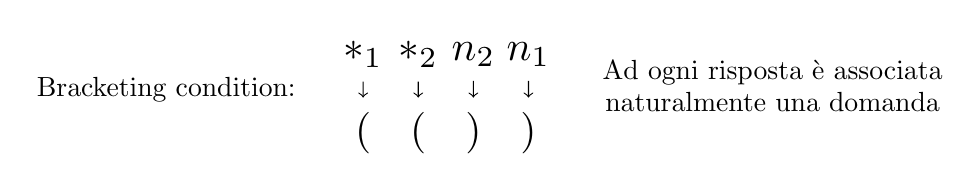
\begin{tikzpicture}
			
			\node (text) at (0,-.45) [minimum size=2pt] {Bracketing condition:};
			\only<9>{
			\node (text2) at (7.7,-.23) [minimum size=2pt] {Ad ogni risposta è associata};
			\node (text3) at (7.7,-.6) [minimum size=2pt] {naturalmente una domanda};
			}
			 \node (st1) at (2.5,0) [minimum size=2pt, scale=1.5] {$*_1$};
			 \node (st2) at (3.2,0) [minimum size=2pt, scale=1.5] {$*_2$};
			 \node (n2) at (3.9,0) [minimum size=2pt, scale=1.5] {$n_2$};
			 \node (n1) at (4.6,0) [minimum size=2pt, scale=1.5] {$n_1$};
			 
			 \node (pst1) at (2.5,-1) [minimum size=2pt, scale=1.5] {$($};
			 \node (pst2) at (3.2,-1) [minimum size=2pt, scale=1.5] {$($};
			 \node (pn2) at (3.9,-1) [minimum size=2pt, scale=1.5] {$)$};
			 \node (pn1) at (4.6,-1) [minimum size=2pt, scale=1.5] {$)$};
			 
			 \draw[->] (st1) to (pst1);
			 \draw[->] (st2) to (pst2);
			 \draw[->] (n1) to (pn1);
			 \draw[->] (n2) to (pn2);
				
			
			 
			  
	\end{tikzpicture}
	
	
	}
	
\end{frame}

% strategie
\begin{frame}

	\frametitle{Strategie}
	
	Una \textbf{strategia} $\sigma$ è un insieme di partite di lunghezza pari (l'ultima mossa è di $P$) tali che:
	\begin{itemize}
		\item<2-> $\sigma$ sia prefix-closed sulle partite di lunghezza pari
		\item<3-> $\sigma$ sia \textit{history free}, cioè
		\begin{itemize}
			\item $sab , tac \in \sigma \Rightarrow b=c$
			\item $sab, t\in \sigma, ta\in P_A \Rightarrow tab\in \sigma$
		\end{itemize}
	\end{itemize}
	
	
	\onslide<4> 
	La condizione di history free, rende le strategie esprimibili tramite una \textit{funzione parziale} a loro associata:
	\begin{gather*}
		    f: M^O \rightharpoonup M^P\\
	            sab\in \sigma \Rightarrow f_\sigma(a)=b\\
	            X=\{ab\;|\;f(a)=b\} \rightarrow \sigma_f=<X> 
	\end{gather*}
	
	
\end{frame}

% esempi di strategie
\begin{frame}

\frametitle{Strategie}

	\begin{columns}
	\begin{column}{0.45\textwidth}
	Gioco $A=( M_A , \lambda_A , P_A , \approx_A )$
		\begin{itemize}
		         	\item $M_{A}=\{*_1,*_2,n_1,n_2\}$
		           	\item $\lambda_{A}= \{ (*_1,OQ) ;$ $ (*_2,PQ) ; (n_1,PA) ; (n_2,OA) \}$
					\item $P_{A}= \{ 
					\epsilon ,$
					$ *_1 ,
					\; *_1n_1, $ 
					$ *_1*_2,
					\; *_1*_2n_2, 
					\; *_1*_2n_2n_1 \}$
					\item $\approx_{A} = id_{A}$        
		\end{itemize}
	\end{column}
	\begin{column}{0.4\textwidth}
		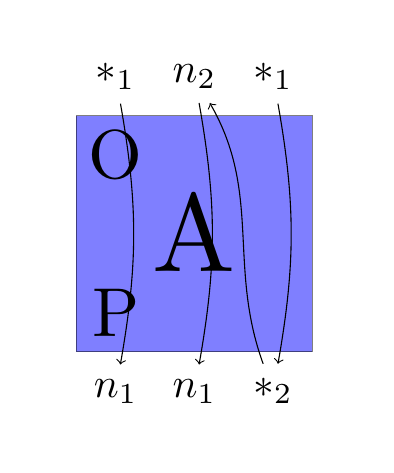
\begin{tikzpicture}
			 \node (inv) at (0,0) [minimum size=2pt] {};
			 \node (inv2) at (4,-5) [minimum size=2pt, scale=1.5] {};
			 
			 \draw [fill=blue, opacity=.5] (3.5,-4) rectangle (.5,-1);
			 \node (A) at (2,-2.5) [minimum size=2pt, scale=4] {A};
			 \node (P) at (1,-3.5) [minimum size=2pt, scale=2.5] {P};
			 \node (O) at (1,-1.5) [minimum size=2pt, scale=2.5] {O};
			 
			 \only<2>{
			 \node (st_12) at (1,-.5) [minimum size=2pt, scale=1.5] {$*_1$};
			 \node (ri_12) at (1,-4.5) [minimum size=2pt, scale=1.5] {$n_1$};
		
			 
			 \node (st_1) at (3,-.5) [minimum size=2pt, scale=1.5] {$*_1$};
			 \node (st_2) at (3,-4.5) [minimum size=2pt, scale=1.5] {$*_2$};
			 \node (ri_1) at (2,-.5) [minimum size=2pt, scale=1.5] {$n_2$};
			 \node (ri_2) at (2,-4.5) [minimum size=2pt, scale=1.5] {$n_1$};
			 
			  \draw[->] [out=280,in=80] (st_1) to (st_2);
			  \draw[->] [out=110,in=300] (st_2) to (ri_1);
			  \draw[->] [out=280,in=80] (ri_1) to (ri_2);
			  \draw[->] [out=280,in=80] (st_12) to (ri_12);
			}
			\end{tikzpicture}
		
	\end{column}
	\end{columns}
	\centering
	\onslide<2>
	Esempi di strategie:
	\begin{gather*}
	\sigma=\{\epsilon, *_1n_1\}\leftrightarrow f_\sigma(*_1)=n_1  \\
	\tau=\{\epsilon, \; *_1*_2, \; *_1*_2n_2n_1\}\leftrightarrow f_\tau(*_1)=*_2,\; f_\tau(n_2)=n_1
	\end{gather*}
	
\end{frame}

% ordine tra strategie
\begin{frame}
 \frametitle{Ordine fra strategie}
 Estendiamo la relazione $\approx$ alle strategie, ponendo:
 \pause
	\begin{itemize}
	\item $\underline{ \sigma \preccurlyeq_s \tau }$ se per ogni $sab \in \sigma$ e $s' \in \tau$ t.c. $sa\approx s'a'$, esiste $b'$ tale che $s'a'b' \in \tau$ e $sab\approx s'a'b'$
	\item $\underline{ \sigma \approx_s \tau \ } \; \text{sse} \; \sigma \preccurlyeq_s \tau \wedge \tau \preccurlyeq_s \sigma$
	\end{itemize}  
	\pause
In particolare, la definizione porta alcune conseguenze: 

	\begin{itemize}
		\item $\preccurlyeq_s$ è un preordine sulle strategie; di conseguenza $\approx_s$ è una relazione di equivalenza parziale
		\item Nel caso l'equivalenza $\approx$ del gioco sia l'identità, l'ordine tra strategie si può vedere come inclusione di insiemi o tra le funzioni parziali. Intuitivamente, $\sigma \preccurlyeq_s \tau$ se $\tau$ può fare più mosse di $\sigma$
	\end{itemize}
	
\end{frame}

% esempio di ordine
\begin{frame}
\frametitle{Ordine fra strategie}
	\begin{columns}
	\begin{column}{0.45\textwidth}
	Gioco $A=( M_A , \lambda_A , P_A , \approx_A )$
		\begin{itemize}
		         	\item $M_{A}=\{*_1,*_2,n_1,n_2\}$
		           	\item $\lambda_{A}= \{ (*_1,OQ) ;$ $ (*_2,PQ) ; (n_1,PA) ; (n_2,OA) \}$
					\item $P_{A}= \{ 
					\epsilon ,$
					$ *_1 ,
					\; *_1n_1, $ 
					$ *_1*_2,
					\; *_1*_2n_2, 
					\; *_1*_2n_2n_1 \}$
					\item $\approx_{A} = id_{A}$        
		\end{itemize}
	\end{column}
	\begin{column}{0.4\textwidth}
		\begin{tikzpicture}
			 \node (inv) at (0,0) [minimum size=2pt] {};
			 \node (inv2) at (4,-5) [minimum size=2pt, scale=1.5] {};
			 
			 \draw [fill=blue, opacity=.5] (3.5,-4) rectangle (.5,-1);
			 \node (A) at (2,-2.5) [minimum size=2pt, scale=4] {A};
			 \node (P) at (1,-3.5) [minimum size=2pt, scale=2.5] {P};
			 \node (O) at (1,-1.5) [minimum size=2pt, scale=2.5] {O};
			 
			 \node (st_12) at (1,-.5) [minimum size=2pt, scale=1.5] {$*_1$};
			 \only<1-2>{\node (ri_12) at (1,-4.5) [minimum size=2pt, scale=1.5] {$n_1$};}
	 		 \only<3-4>{\node (st_22) at (1,-4.5) [minimum size=2pt, scale=1.5] {$*_2$};}
			 \node (st_1) at (3,-.5) [minimum size=2pt, scale=1.5] {$*_1$};
			 \node (st_2) at (3,-4.5) [minimum size=2pt, scale=1.5] {$*_2$};
			 \node (ri_1) at (2,-.5) [minimum size=2pt, scale=1.5] {$n_2$};
			 \node (ri_2) at (2,-4.5) [minimum size=2pt, scale=1.5] {$n_1$};
			 
			  \draw[->] [out=280,in=80] (st_1) to (st_2);
			  \draw[->] [out=110,in=300] (st_2) to (ri_1);
			  \draw[->] [out=280,in=80] (ri_1) to (ri_2);
			  \only<1-2>{\draw[->] [out=280,in=80] (st_12) to (ri_12);}
			  \only<3-4>{\draw[->] [out=280,in=80] (st_12) to (st_22);}
			\end{tikzpicture}
		
	\end{column}
	\end{columns}
	\centering
	\begin{gather*}
	\only<1-2>{\sigma=\{\epsilon, *_1n_1\}\leftrightarrow f_\sigma(*_1)=n_1  \\}
	\only<3-4>{\sigma=\{\only<4>{\textcolor{red}{\epsilon, \; *_1*_2}}\only<3>{\epsilon, \; *_1*_2}\}\leftrightarrow \only<4>{\textcolor{red}{f_\sigma(*_1)=*_2}}\only<3>{f_\sigma(*_1)=*_2}  \\}
	\tau=\{\only<4>{\textcolor{red}{\epsilon, \; *_1*_2}}\only<1-3>{\epsilon, \; *_1*_2}, \; *_1*_2n_2n_1\}\leftrightarrow 
	\only<4>{\textcolor{red}{f_\tau(*_1)=*_2}}\only<1-3>{f_\tau(*_1)=*_2},\; 
	f_\tau(n_2)=n_1
	\\
	\only<2>{\sigma \not\preccurlyeq_s \tau, \; \sigma \not\preccurlyeq_s \tau}
	\only<4>{\sigma \preccurlyeq_s \tau}
	\end{gather*}
\end{frame}

\subsection{operazioni tra giochi}

% prodotto tensore
\begin{frame}
	
	\frametitle{Il gioco $A \otimes B$}
	Dati due giochi $A$ e $B$ definiamo il gioco $A\otimes B$ come:
	\begin{itemize}
		\item<2-> $M_{A\otimes B}=M_A \coprod M_B$
		\item<3-> $\lambda_{A\otimes B}=\lambda_A \coprod \lambda_B$
		\item<4-> $P_{A\otimes B}$ sono tutte le partite $s$ tali che $s|_{M_A} \in P_A \wedge s|_{M_B} \in P_B$
		\begin{itemize}
			\item $s|_{M_A} \in P_A \wedge s|_{M_B} \in P_B$
			\item Per ogni domanda in $A$, la risposta deve essere in $A$; lo stesso con $B$
		\end{itemize}
		\item<5-> $s\approx_{A\otimes B} t \Leftrightarrow s|_A \approx_A t|_A \wedge s|_B \approx_B t|_B \wedge fst(s)=fst(t)$ 
	\end{itemize}
	
	\onslide<6-9>{
	\begin{block}{Proprietà}
		\begin{itemize}
			\item<7-> Il prodotto tensore è associativo
			\item<8-> Esiste un elemento neutro $I$, ossia il gioco vuoto
			\item<9-> \textcolor{red}{Solamente il giocatore $O$ può cambiare componente di gioco}
		\end{itemize}
		
	\end{block}
	}
	
\end{frame}

% esempio Prodotto Tensore
\begin{frame}[t]
\frametitle{Il gioco $A \otimes B$}

\pause
\begin{itemize}
 \item $A$ con $P_A=\{
 \only<3-7>{\textcolor{red}{\epsilon}} \only<1-2,8->{\epsilon},
 \;  \only<8-9>{\textcolor{red}{*_O}} \only<1-7,10->{*_O}, 
 \; \only<10->{\textcolor{red}{*_O\checkmark_P}} \only<1-9>{*_O\checkmark_P}, 
 \;*_O\times_P 
 \}$
 \item $B$ con $P_B=\{
 \only<3>{\textcolor{red}{\epsilon}} \only<1-2,4->{\epsilon},
 \;  \only<4-5>{\textcolor{red}{*_O}} \only<1-3,6->{*_O}, 
 \; *_O0_P,
 \; *_O1_P,
 \; \only<6->{\textcolor{red}{*_O2_P}} \only<1-5>{*_O2_P},
 \; *_O3_P,
 \; \dots \}$
\end{itemize}
\pause
\centering Descriviamo $A \otimes B$ tramite il tavolo di gioco

\begin{tikzpicture}
 
	 \node (inv) at (0,0) [minimum size=2pt] {};
 	 \node (inv2) at (11,-4) [minimum size=2pt] {};
	
	\draw [fill=blue, opacity=.5] (4.5,-4.3) rectangle (1,-.8);
	\draw [fill=red, opacity=.5] (9.5,-4.3) rectangle (6,-.8);
	 
	 \node (tensor) at (5.25,-2.55)[minimum size=2pt, scale=3] {$\otimes$};
	 
	  \node (A) at (2.75,-2.55) [minimum size=2pt, scale=4] {A};
 	  \node (PA) at (1.5,-3.8) [minimum size=2pt, scale=3] {P};
  	  \node (OA) at (1.5,-1.3) [minimum size=2pt, scale=3] {O};
  
	  \node (B) at (7.75,-2.55) [minimum size=2pt, scale=4] {B};
 	  \node (PB) at (6.5,-3.8) [minimum size=2pt, scale=3] {P};
  	  \node (OB) at (6.5,-1.3) [minimum size=2pt, scale=3] {O};
  
	  \only<4-> {\node (st1) at (7.75,-.4) [minimum size=2pt, scale=2] {$*_O$};}
	  \only<5> {\node (false1) at (2.75,-4.7) [minimum size=2pt, scale=2] {?};}
	  \only<6-> {\node (ri1) at (7.75,-4.7) [minimum size=2pt, scale=2] {$2_P$};}
	  \only<7> {\node (false2) at (6.5,-.4) [minimum size=2pt, scale=2] {?};}
	  \only<8-> {\node (st2) at (2.75,-.4) [minimum size=2pt, scale=2] {$*_O$};}
	  \only<9> {\node (false3) at (6.5,-4.7) [minimum size=2pt, scale=2] {?};}
	  \only<10-> {\node (ri2) at (2.75,-4.7) [minimum size=2pt, scale=2] {$\checkmark_P$};}
	 
	 \only<5>{\draw[->] (st1) to (false1);}
	 
	 \only<6->{\draw[->] (st1) to (ri1);}
	 
	 \only<7>{\draw[->] (ri1) to (false2);}
	 
	 \only<8->{\draw[->] (ri1) to (st2);}
	 
	 \only<9>{\draw[->] (st2) to (false3);}
	 
	 \only<10->{\draw[->] (st2) to (ri2);}
	
	 
 
\end{tikzpicture}






	
\end{frame}


% gioco implicazione lineare
\begin{frame}
	
	\frametitle{Il gioco $A \limp B$}
	Dati due giochi $A$ e $B$ definiamo il gioco $A\limp B$ come:
	\begin{itemize}
		\item<2-> $M_{A\limp B}=M_A \coprod M_B$
		\item<3-> $\lambda^{QA}_{A\limp B}=\lambda^{QA}_A \coprod \lambda^{QA}_B$
		
		$\lambda^{OP}_{A\limp B}=\textcolor{red}{\overline{\lambda^{OP}_A}} \coprod \lambda^{OP}_B$
		\item<4-> $P_{A\otimes B}$ sono tutte le partite $s$ tali che:
		\begin{itemize}
			\item $s|_{M_A} \in P_A \wedge s|_{M_B} \in P_B$
			\item Per ogni domanda in $A$, la risposta deve essere in $A$; lo stesso con $B$
		\end{itemize}
		\item<5-> $s\approx_{A\otimes B} t \Leftrightarrow s|_A \approx_A t|_A \wedge s|_B \approx_B t|_B \wedge fst(s)=fst(t)$ 
	\end{itemize}
	\onslide<6>
	\begin{block}{Proprietà}
		
		\textcolor{red}{Solamente il giocatore $P$ può cambiare componente di gioco}
		
	
	\end{block}
	
\end{frame}

% esempio implicazione lineare
\begin{frame}[t]
\frametitle{Il gioco $A \limp B$}

\pause
\begin{itemize}
 \item $A$ con $P_A=\{
 \only<3-6>{\textcolor{red}{\epsilon}} \only<1-2,7->{\epsilon},
 \;  \only<7-8>{\textcolor{red}{*_O}} \only<1-6,9->{*_O}, 
 \; \only<9->{\textcolor{red}{*_O\checkmark_P}} \only<1-8>{*_O\checkmark_P}, 
 \;*_O\times_P 
 \}$
 \item $B$ con $P_B=\{
 \only<3-5>{\textcolor{red}{\epsilon}} \only<1-2,6->{\epsilon},
 \;  \only<6-10>{\textcolor{red}{*_O}} \only<1-5,11->{*_O}, 
 \; *_O0_P,
 \; *_O1_P,
 \; \only<11->{\textcolor{red}{*_O2_P}} \only<1-10>{*_O2_P},
 \; *_O3_P,
 \; \dots \}$
\end{itemize}
\pause
\centering Descriviamo $A \limp B$ tramite il tavolo di gioco

\begin{tikzpicture}
 
	 \node (inv) at (0,0) [minimum size=2pt] {};
 	 \node (inv2) at (11,-4) [minimum size=2pt] {};
	
	\draw [fill=blue, opacity=.5] (4.5,-4.3) rectangle (1,-.8);
	\draw [fill=red, opacity=.5] (9.5,-4.3) rectangle (6,-.8);
	\node (linear) at (5.25,-2.55) [minimum size=2pt, scale=3] {$\limp$};
	 
	  \node (A) at (2.75,-2.55) [minimum size=2pt, scale=4] {A};
	  \only<3>{\node (Pfake) at (1.5,-3.8) [minimum size=2pt, scale=3] {\textcolor{red}{P}};}
  	  \only<3>{\node (Ofake) at (1.5,-1.3) [minimum size=2pt, scale=3] {\textcolor{red}{O}};}
 	  \only<4->{\node (PA) at (2.4,-1.3) [minimum size=2pt, scale=2.7] {P=O$_A$};}
  	  \only<4->{\node (OA) at (2.4,-3.8) [minimum size=2pt, scale=2.7] {O=P$_A$};}
  
	  \node (B) at (7.75,-2.55) [minimum size=2pt, scale=4] {B};
 	  \node (PB) at (6.5,-3.8) [minimum size=2pt, scale=3] {P};
  	  \node (OB) at (6.5,-1.3) [minimum size=2pt, scale=3] {O};
  
          \only<5> {\node (false1) at (2.75,-4.7) [minimum size=2pt, scale=2] {?};}
	  \only<6-> {\node (st1) at (7.75,-.4) [minimum size=2pt, scale=2] {$*_O$};}
	  \only<7-> {\node (st2) at (2.75,-.4) [minimum size=2pt, scale=2] {$*_O$};}
	  \only<8> {\node (false2) at (6.5,-.4) [minimum size=2pt, scale=2] {?};}
	  \only<9-> {\node (ri2) at (2.75,-4.7) [minimum size=2pt, scale=2] {$\checkmark_P$};}
	  \only<10> {\node (false3) at (1.5,-.4) [minimum size=2pt, scale=2] {?};}
	  \only<11-> {\node (ri1) at (7.75,-4.7) [minimum size=2pt, scale=2] {$2_P$};}
	  
	  
	 
	 \only<7->{\draw[->][out=220, in=340] (st1) to (st2);}
	 \only<8>{\draw[->] (st2) to (false2);}
	 \only<9->{\draw[->] (st2) to (ri2);}
	 \only<10>{\draw[->] (ri2) to (false3);}
	 \only<11->{\draw[->] (ri2) to (ri1);}
	 

	
	 
 
\end{tikzpicture}






	
\end{frame}

% gioco prodotto tensore infinito
\begin{frame}
	
	\frametitle{Il gioco $!A$}
	
	\begin{itemize}
		\item $M_{!A}=\omega \times M_A$
		\item $\lambda_{!A}(i,a)=\lambda_A(a)$
		\item $s$ è una partita di $P_{!A}$ se e solo se:
		\begin{itemize}
			\item $\forall i\in \omega , s|_i \in P_A$
			\item Se una domanda è nella componente $i$, la sua risposta deve essere nella componente $i$ (\emph{indexed bracketing condition})
		\end{itemize}

		\item $s\approx_{!A} t$ sse esiste $\pi:\omega \rightarrow \omega$ permutazione tale che $s|_i \approx_A t|_{\pi(i)} \wedge (\pi \circ fst)(s)=fst(t)$
	\end{itemize}
	
	\begin{block}{Proprietà}
		\begin{itemize}
			\item Solamente il giocatore $O$ può cambiare componente di gioco
		\end{itemize}
	\end{block}
	
	Nota: concettualmente il gioco $!A$ si comporta come se avessimo infinite copie di $A$ tensorizzate $A\otimes A\otimes A\otimes A\otimes \dots$ con la relazione $\approx_{!A}$
	
\end{frame}

% roulette russa
\begin{frame}
\frametitle{Il gioco $A\Rightarrow B$}

\only<2->{
	\[
	A \Rightarrow B \quad \equiv \quad !A \limp B
	\]
}

\only<1-10>{
\onslide<3->{
\begin{itemize}
 \item $Gun=A$ con $P_A=\{
 \only<3-5>{\textcolor{red}{\epsilon}} \only<1-2,6->{\epsilon},
 \;  \only<6,8>{\textcolor{red}{\underline{pull}}} \only<1-5,7,9->{\underline{pull}}, 
 \; \only<7>{\textcolor{red}{\underline{pull}\:click}} \only<1-6,8->{\underline{pull}\:click}, 
 \; \only<9->{\textcolor{red}{\underline{pull}\:bang}} \only<1-8>{\underline{pull}\:bang} 
 \}$
 \item $Life=B$ con $P_B=\{
 \only<3-4>{\textcolor{red}{\epsilon}} \only<1-2,5->{\epsilon},
 \;  \only<5-9>{\textcolor{red}{*_O}} \only<1-4,10->{*_O}, 
 \; *_O\checkmark_P,
 \; *_O1_P,
 \; \only<10->{\textcolor{red}{*_O2_P}} \only<1-9>{*_O2_P},
 \; *_O3_P,
 \; \dots \}$
 \item<4-> Strategia \textit{Roulette Russa}:
 
 $\only<6>{\textcolor{red}{f(*_O)=\underline{pull}_1}} \only<4-5,7->{f(*_O)=\underline{pull}_1}$, 
 $\quad \only<8>{\textcolor{red}{f(click_n)=\underline{pull}_{n+1}}} \only<4-7,9->{f(click_n)=\underline{pull}_{n+1}} \forall n$,  
 $\quad \only<10>{\textcolor{red}{f(bang_n)=n_P}} \only<4-9>{f(bang_n)=n_P}$
\end{itemize}
}
}


\only<11->{

\begin{itemize}
 \item $Gun=A$ con $P_A=\{
 \only<3-5>{\textcolor{red}{\epsilon}} \only<1-2,6->{\epsilon},
 \;  \only<6,8>{\textcolor{red}{\underline{pull}}} \only<1-5,7,9->{\underline{pull}}, 
 \; \only<7>{\textcolor{red}{\underline{pull}\:click}} \only<1-6,8->{\underline{pull}\:click}, 
 \; \only<9->{\textcolor{red}{\underline{pull}\:bang}} \only<1-8>{\underline{pull}\:bang} 
 \}$
 \item $Life=B$ con $P_B=\{
 \only<3-4>{\textcolor{red}{\epsilon}} \only<1-2,5->{\epsilon},
 \;  \only<5-9>{\textcolor{red}{*_O}} \only<1-4,10->{*_O}, 
 \; *_O\checkmark_P,
 \; *_O1_P,
 \; \only<10->{\textcolor{red}{*_O2_P}} \only<1-9>{*_O2_P},
 \; *_O3_P,
 \; \dots \}$
 \item Strategia \textit{Roulette Russa}:
 
 $\only<6>{\textcolor{red}{f(*_O)=\underline{pull}_2}} \only<4-5,7->{f(*_O)=\underline{pull}_2}$, 
 $\quad \only<8>{\textcolor{red}{f(click_{2n})=\underline{pull}_{2n+2}}} \only<4-7,9->{f(click_{2n})=\underline{pull}_{2n+2}} \forall n$,  
 $\quad \only<10->{\textcolor{red}{f(bang_{2n})=n_P}} \only<4-9>{f(bang_{2n})=n_P}$
\end{itemize}

}



\only<2-10>{ 
	\begin{tikzpicture}
	 \node (inv) at (0,0) [minimum size=2pt] {};
	 \node (inv2) at (11,-4) [minimum size=2pt] {};
	 \foreach \x in {0,3,6} { 
	  \draw [fill=blue, opacity=.5] (\x+2,-3) rectangle (\x,-1);
	 % \node (A) at (\x+1,-2) [minimum size=2pt, scale=2] {A};
	  \node (P) at (\x+0.3,-1.3) [minimum size=2pt, scale=1.5] {P};
 	  \node (O) at (\x+0.3,-2.7) [minimum size=2pt, scale=1.5] {O};
	  }
	  \node (A) at (7,-2) [minimum size=2pt, scale=2] {A$_1$};
	  \node (A) at (4,-2) [minimum size=2pt, scale=2] {A$_2$};
	  \node (A) at (1,-2) [minimum size=2pt, scale=2] {A$_3$};
	 \draw [fill=red, opacity=.5] (11,-3) rectangle (9,-1);
	 \node (B) at (10,-2) [minimum size=2pt, scale=2] {B};
	 \node (P) at (9.3,-2.7) [minimum size=2pt, scale=1.5] {P};
 	 \node (O) at (9.3,-1.3) [minimum size=2pt, scale=1.5] {O};
	 
	 \node (linear) at (8.5,-2) [minimum size=2pt, scale=1.5] {$\limp$};
	 \node (tensor1) at (5.5,-2) [minimum size=2pt, scale=1.5] {$\otimes$};
	 \node (tensor2) at (2.5,-2) [minimum size=2pt, scale=1.5] {$\otimes$};
	 
	 \only<5->{\node (st1) at (10,-0.5) [minimum size=2pt, scale=1.5] {$*_O$};}
 	 \only<6->{\node (st2) at (7,-0.5) [minimum size=2pt, scale=1.5] {$\underline{pull}_1$};}
	 \only<7->{\node (ri2) at (7,-3.5) [minimum size=2pt, scale=1.5] {$click_1$};}
 	 \only<8->{\node (st3) at (4,-0.5) [minimum size=2pt, scale=1.5] {$\underline{pull}_2$};}
	 \only<9->{\node (ri3) at (4,-3.5) [minimum size=2pt, scale=1.5] {$bang_2$};}
 	 \only<10->{\node (ri1) at (10,-3.5) [minimum size=2pt, scale=1.5] {$2_P$};}
 	 
	  \only<6->{\draw[->] [out=250,in=280] (st1) to (st2);}
	  \only<7->{\draw[->] [out=250,in=30] (st2) to (ri2);}
	  \only<8->{\draw[->] [out=80,in=280] (ri2) to (st3);}
	  \only<9->{\draw[->] [out=250,in=110] (st3) to (ri3);}
	  \only<10->{\draw[->] [out=30,in=150] (ri3) to (ri1);}
	  \end{tikzpicture}

	}

	
\only<11->{ 
	\begin{tikzpicture}
	 \node (inv) at (0,0) [minimum size=2pt] {};
	 \node (inv2) at (11,-4) [minimum size=2pt] {};
	 \foreach \x in {0,3,6} { 
	  \draw [fill=blue, opacity=.5] (\x+2,-3) rectangle (\x,-1);
	 % \node (A) at (\x+1,-2) [minimum size=2pt, scale=2] {A};
	  \node (P) at (\x+0.3,-1.3) [minimum size=2pt, scale=1.5] {P};
 	  \node (O) at (\x+0.3,-2.7) [minimum size=2pt, scale=1.5] {O};
	  }
	  \node (A) at (7,-2) [minimum size=2pt, scale=2] {A$_2$};
	  \node (A) at (4,-2) [minimum size=2pt, scale=2] {A$_4$};
	  \node (A) at (1,-2) [minimum size=2pt, scale=2] {A$_6$};
	 \draw [fill=red, opacity=.5] (11,-3) rectangle (9,-1);
	 \node (B) at (10,-2) [minimum size=2pt, scale=2] {B};
	 \node (P) at (9.3,-2.7) [minimum size=2pt, scale=1.5] {P};
 	 \node (O) at (9.3,-1.3) [minimum size=2pt, scale=1.5] {O};
	 
	 \node (linear) at (8.5,-2) [minimum size=2pt, scale=1.5] {$\limp$};
	 \node (tensor1) at (5.5,-2) [minimum size=2pt, scale=1.5] {$\otimes$};
	 \node (tensor2) at (2.5,-2) [minimum size=2pt, scale=1.5] {$\otimes$};
	 
	 \only<5->{\node (st1) at (10,-0.5) [minimum size=2pt, scale=1.5] {$*_O$};}
 	 \only<6->{\node (st2) at (7,-0.5) [minimum size=2pt, scale=1.5] {$\underline{pull}_2$};}
	 \only<7->{\node (ri2) at (7,-3.5) [minimum size=2pt, scale=1.5] {$click_2$};}
 	 \only<8->{\node (st3) at (4,-0.5) [minimum size=2pt, scale=1.5] {$\underline{pull}_4$};}
	 \only<9->{\node (ri3) at (4,-3.5) [minimum size=2pt, scale=1.5] {$bang_4$};}
 	 \only<10->{\node (ri1) at (10,-3.5) [minimum size=2pt, scale=1.5] {$2_P$};}
 	 
	  \only<6->{\draw[->] [out=250,in=280] (st1) to (st2);}
	  \only<7->{\draw[->] [out=250,in=30] (st2) to (ri2);}
	  \only<8->{\draw[->] [out=80,in=280] (ri2) to (st3);}
	  \only<9->{\draw[->] [out=250,in=110] (st3) to (ri3);}
	  \only<10->{\draw[->] [out=30,in=150] (ri3) to (ri1);}
	  \end{tikzpicture}

	}
	
\end{frame}


\subsection{strategie importanti}

% strategia composizione con esempio
\begin{frame}

	\frametitle{La strategia $\sigma ; \tau$}
Date $\sigma$ strategia di $A\limp B$ e $\tau$ di $B\limp C$, allora

\begin{itemize}
 \item<2-> $\sigma ; \tau =\{s|_{A,C} : s \in (M_A \coprod M_B \coprod M_C)^*, \; s|_{A,B} \in \sigma, \; s|_{B,C} \in \tau \}$
 \item<3-> $\sigma ; \tau$ è una strategia di $A\limp C$
\end{itemize}

\onslide<4->{Si può dare una costruzione di $\sigma ; \tau$ algoritmica:}

\only<-13>{
\begin{tikzpicture}
			 \node (inv) at (0,0) [minimum size=2pt] {};
			 \node (inv2) at (11,-5) [minimum size=2pt, scale=1.5] {};
			
			\only<5->{
			 \draw [fill=blue, opacity=.5] (1.9,-3.5) rectangle (-.1,-1.5);
			 \draw [fill=red, opacity=.5] (4.9,-3.5) rectangle (2.9,-1.5);
			 \draw [fill=red, opacity=.5] (7.4,-3.5) rectangle (5.4,-1.5);
			 \draw [fill=green, opacity=.5] (10.4,-3.5) rectangle (8.4,-1.5);
			 			 
			 \node (A) at (.9,-2.5) [minimum size=2pt, scale=2] {A};
			 \node (B) at (3.9,-2.5) [minimum size=2pt, scale=2] {B};
			 \node (B) at (6.4,-2.5) [minimum size=2pt, scale=2] {B};
			 \node (C) at (9.4,-2.5) [minimum size=2pt, scale=2] {C};
			 
			 \node (P) at (.2,-1.8) [minimum size=2pt, scale=1.5] {P};
			 \node (P) at (3.2,-3.2) [minimum size=2pt, scale=1.5] {P};
			 \node (P) at (5.7,-1.8) [minimum size=2pt, scale=1.5] {P};
			 \node (P) at (8.7,-3.2) [minimum size=2pt, scale=1.5] {P};
			 
			 \node (O) at (.2,-3.2) [minimum size=2pt, scale=1.5] {O};
			 \node (O) at (3.2,-1.8) [minimum size=2pt, scale=1.5] {O};
			 \node (O) at (5.7,-3.2) [minimum size=2pt, scale=1.5] {O};
			 \node (O) at (8.7,-1.8) [minimum size=2pt, scale=1.5] {O};
			 
			 \node (linear1) at (2.4,-2.5) [minimum size=2pt, scale=1.5] {$\limp$};
			 \node (linear2) at (7.9,-2.5) [minimum size=2pt, scale=1.5] {$\limp$};
			
			 
			 \node (sigma) at (2.3,-.3) [minimum size=2pt, scale=2] {\only<8,10,12>{\textcolor{red}{$\sigma$}} \only<1-7,9,11,13>{$\sigma$}};
			 \node (tau) at (7.9,-.3) [minimum size=2pt, scale=2] {\only<7,9,13>{\textcolor{red}{$\tau$}} \only<1-6,8,10-12>{$\tau$}};
			\draw[dashed] (5.15, -4.5) -- (5.15, -.5);
			}
			
			
			\only<6->{ \node (st_1) at (9.4,-1) [minimum size=2pt, scale=1.5] {$*_1$};}
			\only<7->{\node (st_2) at (6.9,-1) [minimum size=2pt, scale=1.5] {$*_2$};}
			 \only<7->{\node (st_2b) at (4.4,-1) [minimum size=2pt, scale=1.5] {$*_2$};}
			\only<8->{  \node (ri_2) at (6.9,-4) [minimum size=2pt, scale=1.5] {$n_2$};}
			 \only<8->{ \node (ri_2b) at (4.4,-4) [minimum size=2pt, scale=1.5] {$n_2$};}
			 \only<9->{\node (st_3) at (5.9,-1) [minimum size=2pt, scale=1.5] {$*_3$};}
			\only<9->{ \node (st_3b) at (3.4,-1) [minimum size=2pt, scale=1.5] {$*_3$};}
			 \only<10->{\node (st_4) at (.9,-1) [minimum size=2pt, scale=1.5] {$*_4$};}
			 \only<11->{\node (ri_4) at (.9,-4) [minimum size=2pt, scale=1.5] {$n_4$};}
			 \only<12->{\node (ri_3b) at (3.4,-4) [minimum size=2pt, scale=1.5] {$n_3$};}
			\only<12->{ \node (ri_3) at (5.9,-4) [minimum size=2pt, scale=1.5] {$n_3$};}
			\only<13->{ \node (ri_1) at (9.4,-4) [minimum size=2pt, scale=1.5] {$n_1$};}
			 
			 %\node (ri_2) at (2,-4.5) [minimum size=2pt, scale=1.5] {$n_1$};
			 
			 \only<7->{ \draw[->] (st_1) to (st_2);}
			  \only<8->{\draw[dashed,->] (st_2) to (ri_2);}
			  \only<8->{\draw[->] (st_2b) to (ri_2b);}
			  \only<9->{\draw[->] (ri_2) to (st_3);}
			 \only<9->{ \draw[dashed,->] (ri_2b) to (st_3b);}
			\only<10->{  \draw[->] (st_3b) to (st_4);}
			 \only<11->{ \draw[->] (st_4) to (ri_4);}
			 \only<12->{ \draw[dashed,->] (st_3) to (ri_3);}
			 \only<12->{ \draw[->] (ri_4) to (ri_3b);}
			 \only<13->{ \draw[->] [in=150, out=30] (ri_3) to (ri_1);}
			  
			  %\draw[->] [out=180,in=300] (st_2) to (ri_1);
			  %\draw[->] [out=280,in=0] (ri_1) to (ri_2);
			
			\end{tikzpicture}
}

\only<14->{
\begin{tikzpicture}
			 \node (inv) at (0,0) [minimum size=2pt] {};
			 \node (inv2) at (11,-5) [minimum size=2pt, scale=1.5] {};
			
			\only<5->{
			 \draw [fill=blue, opacity=.5] (1.9,-3.5) rectangle (-.1,-1.5);
			 \draw [fill=red, opacity=.1] (4.9,-3.5) rectangle (2.9,-1.5);
			 \draw [fill=red, opacity=.1] (7.4,-3.5) rectangle (5.4,-1.5);
			 \draw [fill=green, opacity=.5] (10.4,-3.5) rectangle (8.4,-1.5);
			 			 
			 \node (A) at (.9,-2.5) [minimum size=2pt, scale=2] {A};
			 \node (B) at (3.9,-2.5) [opacity=.1, minimum size=2pt, scale=2] {B};
			 \node (B) at (6.4,-2.5) [opacity=.1, minimum size=2pt, scale=2] {B};
			 \node (C) at (9.4,-2.5) [minimum size=2pt, scale=2] {C};
			 
			 \node (P) at (.2,-1.8) [minimum size=2pt, scale=1.5] {P};
			 \node (P) at (3.2,-3.2) [opacity=.1, minimum size=2pt, scale=1.5] {P};
			 \node (P) at (5.7,-1.8) [opacity=.1, minimum size=2pt, scale=1.5] {P};
			 \node (P) at (8.7,-3.2) [minimum size=2pt, scale=1.5] {P};
			 
			 \node (O) at (.2,-3.2) [minimum size=2pt, scale=1.5] {O};
			 \node (O) at (3.2,-1.8) [opacity=.1, minimum size=2pt, scale=1.5] {O};
			 \node (O) at (5.7,-3.2) [opacity=.1, minimum size=2pt, scale=1.5] {O};
			 \node (O) at (8.7,-1.8) [minimum size=2pt, scale=1.5] {O};
			 
			  \node (linear1) at (2.4,-2.5) [opacity=.1, minimum size=2pt, scale=1.5] {$\limp$};
			 \node (linear2) at (7.9,-2.5) [opacity=.1, minimum size=2pt, scale=1.5] {$\limp$};
			  \node (linear3) at (5.15,-2.5) [, minimum size=2pt, scale=2] {$\limp$};
			 			 
			 \node (sigma) at (2.3,-.3) [minimum size=2pt, scale=2] {\only<8,10,12>{\textcolor{red}{$\sigma$}} \only<1-7,9,11,13>{$\sigma$}};
			 \node (tau) at (7.9,-.3) [minimum size=2pt, scale=2] {\only<7,9,13>{\textcolor{red}{$\tau$}} \only<1-6,8,10-12>{$\tau$}};
			\draw[opacity=.1, dashed] (5.15, -4.5) -- (5.15, -.5);
			}
			
			\node (st) at (5.15, -.3)[minimum size=2pt, scale=2] {$\sigma ; \tau$};
			
			
			\only<6->{ \node (st_1) at (9.4,-1) [minimum size=2pt, scale=1.5] {$*_1$};}
			\only<7->{\node (st_2) at (6.9,-1) [opacity=.1, minimum size=2pt, scale=1.5] {$*_2$};}
			 \only<7->{\node (st_2b) at (4.4,-1) [opacity=.1, minimum size=2pt, scale=1.5] {$*_2$};}
			\only<8->{  \node (ri_2) at (6.9,-4) [opacity=.1, minimum size=2pt, scale=1.5] {$n_2$};}
			 \only<8->{ \node (ri_2b) at (4.4,-4) [opacity=.1, minimum size=2pt, scale=1.5] {$n_2$};}
			 \only<9->{\node (st_3) at (5.9,-1) [opacity=.1, minimum size=2pt, scale=1.5] {$*_3$};}
			\only<9->{ \node (st_3b) at (3.4,-1) [opacity=.1, minimum size=2pt, scale=1.5] {$*_3$};}
			 \only<10->{\node (st_4) at (.9,-1) [minimum size=2pt, scale=1.5] {$*_4$};}
			 \only<11->{\node (ri_4) at (.9,-4) [minimum size=2pt, scale=1.5] {$n_4$};}
			 \only<12->{\node (ri_3b) at (3.4,-4) [opacity=.1, minimum size=2pt, scale=1.5] {$n_3$};}
			\only<12->{ \node (ri_3) at (5.9,-4) [opacity=.1, minimum size=2pt, scale=1.5] {$n_3$};}
			\only<13->{ \node (ri_1) at (9.4,-4) [minimum size=2pt, scale=1.5] {$n_1$};}
			 
			 %\node (ri_2) at (2,-4.5) [minimum size=2pt, scale=1.5] {$n_1$};
			 
			 \only<7->{ \draw[opacity=.1, ->] (st_1) to (st_2);}
			  \only<8->{\draw[opacity=.1, dashed,->] (st_2) to (ri_2);}
			  \only<8->{\draw[opacity=.1, ->] (st_2b) to (ri_2b);}
			  \only<9->{\draw[opacity=.1, ->] (ri_2) to (st_3);}
			 \only<9->{ \draw[opacity=.1, dashed,->] (ri_2b) to (st_3b);}
			\only<10->{  \draw[opacity=.1, ->] (st_3b) to (st_4);}
			 \only<11->{ \draw[->] (st_4) to (ri_4);}
			 \only<12->{ \draw[opacity=.1, dashed,->] (st_3) to (ri_3);}
			 \only<12->{ \draw[opacity=.1, ->] (ri_4) to (ri_3b);}
			 \only<13->{ \draw[opacity=.1, ->] [in=150, out=30] (ri_3) to (ri_1);}
			 
			 \draw[->] [in=360, out=200] (st_1) to (st_4);
			 \draw[->] [in=160, out=20] (ri_4) to (ri_1);
			  
			  %\draw[->] [out=180,in=300] (st_2) to (ri_1);
			  %\draw[->] [out=280,in=0] (ri_1) to (ri_2);
			
			\end{tikzpicture}
	}		
			
\end{frame}


% strategia copycat
\begin{frame}

	\frametitle{La strategia \emph{copycat} su $A\limp A$}
Dato $A$, è sempre possibile costruire la strategia \emph{copycat} su $A\limp A$:

\begin{itemize}
 \item<2-> $id_A=\{s \in P_{A\limp A} : s|_1=s|_2 \}$ 
 \item<3-> la strategia consiste nel copiare le mosse di $O$ sull'altra componente, quindi la funzione parziale associata a questa strategia è
 \[
 f(x_1)=x_2, \quad f(x_2)=x_1 \quad \forall x \in M_A
 \]
 \item<4-> Data $\sigma$ strategia di $A\limp B$, avremo che $id_A;\sigma=\sigma$
\end{itemize}


\end{frame}


\subsection{esistenza del modello}

% categoria dei giochi
\begin{frame}
 	
 	\frametitle{La categoria dei giochi $\mathcal{G}$}
 	
 	Definiamo $\mathcal{G}$ la categoria tale che:
 	\begin{itemize}
 		\item<2-> $\mathcal{G}_0$ sono i giochi
 		\item<3-> dati due giochi $A$ e $B$, i morfismi $A\rightarrow B$ sono $\{ \sigma \text{ strategia di } A\limp B \;|\; \sigma \approx_s \sigma \} / \approx_s$
 		\item<4-> Date $[\sigma] : A\rightarrow B$ e $[\tau] : B \rightarrow C$, $[\tau] \circ [\sigma] = [\sigma ; \tau]$
		\item<5-> Il morfismo identico è dato dalla strategia $id_A$
 	\end{itemize}
 	
 	\onslide<6->{In particolare abbiamo che $\mathcal{G}$:}
 	\begin{itemize}
 		\item<7-> è dotata di un oggetto finale ($1$)
 		\item<8-> è una categoria monoidale 
 		
 		($\otimes$ è un bifuntore associativo con elemento neutro)
 		\item<9-> è una categoria autonoma 
 		
 		(per ogni gioco $A$ esiste il suo gioco duale $1 \limp A$)
 		\item<10-> NON è una categoria cartesiana chiusa (mancano i prodotti)
 	\end{itemize}
 	
 \end{frame}

 % gioco unione
\begin{frame}
	
	\frametitle{Il gioco $A \& B$}
	Dati due giochi $A$ e $B$ definiamo il gioco $A\& B$ come:
	\begin{itemize}
		\item<2-> $M_{A\& B}=M_A \coprod M_B$
		\item<2-> $\lambda_{A\& B}=\lambda_A \coprod \lambda_B$
		\item<2-> $P_{A\& B}=P_A \coprod P_B$
		\item<2-> $\approx_{A\& B} \; = \; \approx_A \coprod \approx_B$ 
	\end{itemize}
	
	\onslide<3->{
	\begin{block}{Proprietà}
		\begin{itemize}
			\item<4-> Una partita di $A\& B$ è giocata su una sola delle due componenti
			\item<5-> Ogni strategia di $A\& B$ è unione di una strategia di $A$ e di una strategia di $B$ (anche vuota)
		\end{itemize}	
	\end{block}
	}
\end{frame}

% dag e der
\begin{frame}
\frametitle{strategie $der$ e $\dag$}

Dato un gioco $A$, definiamo la strategia $der$ su $!A\limp A$:
\begin{itemize}
 \item<2-> Se $A_i$ è l'$i$-esima componente di $!A$, allora $der_A^i$ si comporta come la strategia copycat su $A_i\limp A \;\cong\; A\limp A$, e non agisce sulle altre componenti 
 \item<3-> Dato che le componenti di $!A$ sono equivalenti, avremo che $der_A^i\approx_s der_A^j \: \forall i,j$ , quindi lo indicheremo semplicemente con $der_A$  
\end{itemize}

\onslide<4->{
Data una strategia $\sigma$ su $!A\limp B$, definiamo la strategia $\sigma^{\dag}$ su $!A\limp !B$:
}

\onslide<5->{
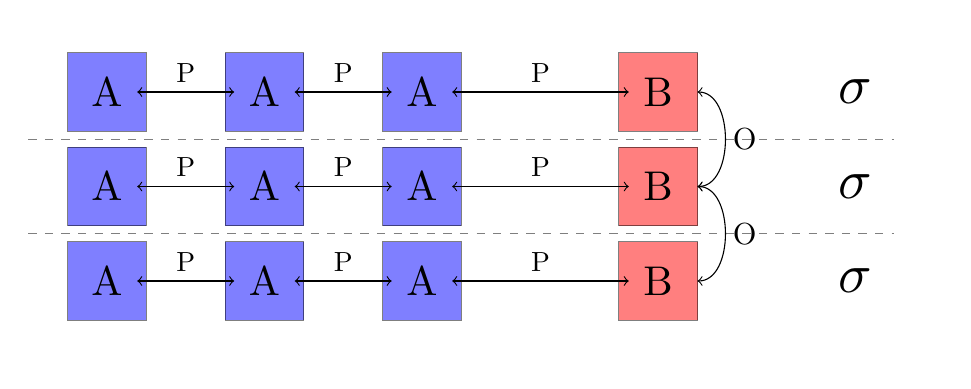
\begin{tikzpicture}
 
 \node (inv) at (0,0) [minimum size=2pt] {};
	 \node (inv2) at (11,-4) [minimum size=2pt] {};
	 
	 \foreach \y in {0,-1.2,-2.4} {
  \foreach \x in {0,2,4} { 
	  \draw [fill=blue, opacity=.5] (\x+1,\y-1.2) rectangle (\x,\y-.2);
	  \node (A\x) at (\x+.5,\y-.7) [minimum size=2pt, scale=1.5] {A};
	  }
	  \draw [<->] (A0) -- (A2)  node [above,midway] {P} ;
	  \draw [<->] (A2) -- (A4)  node [above,midway] {P} ;

 \draw [fill=red, opacity=.5] (8,\y-1.2) rectangle (7,\y-.2);
	 \node (B) at (7.5,\y-.7) [minimum size=2pt, scale=1.5] {B};
	 \node (s) at (10,\y-.7) [minimum size=2pt, scale=2] {$\sigma$};
	 \draw [<->] (A4) -- (B)  node [above,midway] {P} ;

 }
 
 \draw [<->] [out=0,in=0] (8,-1.9) to (8,-3.1) ;
 \draw [<->] [out=0,in=0] (8,-1.9) to (8,-.7) ;
 \node (O) at (8.6,-2.5) [minimum size=2pt, scale=1.1] {O};
 \node (O) at (8.6,-1.3) [minimum size=2pt, scale=1.1] {O};
 \draw[opacity=.5, dashed] (-.5, -1.3) -- (10.5, -1.3);
 \draw[opacity=.5, dashed] (-.5, -2.5) -- (10.5, -2.5);
 \end{tikzpicture}
}

\end{frame}

% categoria di co-Kleisli
\begin{frame}
\frametitle{categoria di co-Kleisli}
\onslide<2->{
Definiamo $K_!(\mathcal{G})$ la categoria di \emph{co-Kleisli} di $\mathcal{G}$ rispetto a $!$

In particolare:
	}
	\begin{itemize}
		\item<3-> $K_!(\mathcal{G})_0 = \mathcal{G}_0$
		\item<4-> Dati due giochi $A,B$, $Mor_{K_!(\mathcal{G})}(A,B) = Mor_{\mathcal{G}}(!A,B)$
		\item<5-> Date due strategie $\sigma$ e $\tau$, $\tau \circ \sigma = \sigma \fatsemi \tau := \sigma ^\dag ; \tau$
		\item<6-> Dato un gioco $A$, il morfismo identico è $der_A$
	\end{itemize}

	\onslide<7->{In particolare $K_!(\mathcal{G})$ è una \emph{categoria cartesiana chiusa}, cioè:}
	\begin{itemize}
		\item<8-> Dati due oggetti esiste il \emph{prodotto} ($A\& B$)
		\item<9-> Esiste un oggetto \emph{finale} ($1$)
		\item<10-> Dati due oggetti, esiste l'oggetto esponente 
		
		(``$\Rightarrow$'' è tale che $Mor_{K_!(\mathcal{G})}(A\& B,C) \cong Mor_{K_!(\mathcal{G})}(A,B\Rightarrow C)$)
	\end{itemize}

\end{frame}

% ppo e ccc razionale
\begin{frame}
	
	\frametitle{order enrichement e razionalità}
	\onslide<2->{
	Definiamo un \emph{pointed poset (ppo)} come un poset con un minimo (generalmente indicato con $\perp$)
	}
	\onslide<3->{
	Definiamo una categoria cartesiana chiusa $C$ \emph{pointed poset enriched} se:}
	\begin{itemize}
		\item<4-> Dati due oggetti $A,B$, $(Mor(A,B),\sqsubseteq _{A,B},\perp _{A,B})$ è un pointed poset
		\item<5-> Composizione, prodotto e currying sono monotoni
		\item<6-> Per ogni $f: A\rightarrow B$, per ogni gioco $C$, $\perp_{B,C} \circ f = \perp _{A,B}$
	\end{itemize}
	\onslide<7->{
	Definiamo una categoria cartesiana chiusa $C$ \emph{razionale} se:
	}
	\begin{itemize}
		\item<8-> è ppo-enriched
		\item<9-> per ogni $f: A\times B \rightarrow B$ si ha:
		\begin{itemize}
			\item La catena $(f^{(k)} | k\in \omega)$ definita da $f^{(0)}=\perp _{A,B}$ e $f^{k+1} = f \circ <id_A , f^{(k)}>$ ammette \emph{least upper bound} $f^{\triangledown}$
			\item Dati $g:C\rightarrow A$ e $h:B\rightarrow D$, $g\circ f^\triangledown \circ h = \bigsqcup_{k\in \omega} g \circ f^{(k)} \circ h$
		\end{itemize}

	\end{itemize}
	
\end{frame}

% I giochi sono un modello di PCF
\begin{frame}
	\frametitle{Denotazione di PCF}
	\onslide<2->{
	Dato $A$ gioco, date $[\sigma],[\tau]$ classi di strategie di $A$, definiamo
	\[[\sigma] \sqsubseteq [\tau] \Leftrightarrow \sigma \preccurlyeq_s \tau\]
	}
	\onslide<3->{
	\begin{block}{Teorema}
		$K_! (\mathcal{G})$ con l'ordine $\sqsubseteq$ è razionale
	\end{block}
	}
	\onslide<4->{
	\begin{block}{Teorema}
		Sia $C$ una categoria cartesiana chiusa razionale. Si ha che:
		\begin{itemize}
			\item Fissata la denotazione dei tipi base di PCF in $C$ (ogni tipo viene denotato con un oggetto)
			\item Fissata la denotazione delle costanti di PCF in $C$ (ogni termine di tipo $\tau$ viene denotato con un morfismo di $1\rightarrow \llbracket \tau \rrbracket$)
		\end{itemize}
		allora la denotazione può essere estesa a tutti i termini di PCF
		
	\end{block}
	}
\end{frame}


\section{Il modello di Abramsky}

\subsection{Denotazione di PCF}

% interpretazioni di tipi
\begin{frame}
	
		
	\begin{block}{example}
		\begin{description}
			\item[$Bool$] \begin{itemize}
			              	\item $M_{Bool}=\{*,t,f\}$
			              	\item $\lambda_{Bool}= \{ (*,OQ) ; (t,PA) ; (f,PA) \}$
			              	\item $P_{Bool}= \{ \epsilon , * ,*t, *f \}$
			              	\item $\approx_{Bool} = id_{Bool}$
			              \end{itemize}

			\item[$Nat$] \begin{itemize}
			              	\item $M_{Nat}=\{ * , \underline{0} , \underline{1} , \dots \}$
			              	\item $\lambda_{Nat}= \{ (*,OQ) , (\underline{0},PA) , (\underline{1},PA) , \dots \}$
			              	\item $P_{Nat}= \{ \epsilon , * , *\underline{0} , *\underline{1} , \dots \}$
											\item $\approx_{Nat} = id_{Nat}$
			              \end{itemize}
		\end{description}

	\end{block}	
	
\end{frame}


% interpretazione di termini semplici
\begin{frame}
	
	\frametitle{Interpretazione dei termini}
	
	Per poter usare il teorema prima dobbiamo fissare la denotazione dei giochi e delle costanti
	Indichiamo con $\llbracket \cdot \rrbracket$ la denotazione
	
	\begin{block}{Tipi}
		
		La denotazione di un tipo è un gioco
		
		\begin{itemize}
			\item $\llbracket Bool \rrbracket = Bool$
			\item $\llbracket Nat \rrbracket = Nat$
			\item $\llbracket S \times T \rrbracket = \llbracket S \rrbracket \& \llbracket T \rrbracket$
			\item $\llbracket S \rightarrow T \rrbracket = \llbracket S \rrbracket \Rightarrow \llbracket T \rrbracket$
		\end{itemize}
	\end{block}
	
	
	
\end{frame}

% interpretazione di termini complessi
\begin{frame}
	
	\begin{block}{Termini}
		
		\small
		
		La denotazione di un termine di tipo $T$ è una strategia di $(1\& A_1 \& \dots \& A_n)\rightarrow T$
		
		\begin{itemize}
			\item $\llbracket true : Bool \rrbracket = \sigma_{tt} : 1 \rightarrow Bool$
			\item $\llbracket false : Bool \rrbracket = \sigma_{ff} : 1 \rightarrow Bool$
			\item $\llbracket n : Nat \rrbracket = \sigma_n : 1 \rightarrow Nat$
			\item $\llbracket M + N \rrbracket = < \sigma_{add} , < \llbracket M \rrbracket , \llbracket N \rrbracket > > \fatsemi \; App$
			\item $\llbracket Eq? M N \rrbracket = < \sigma_{eq} , < \llbracket M \rrbracket , \llbracket N \rrbracket > > \fatsemi \; App$
			\item $\llbracket < s ,t > \rrbracket = <\llbracket s \rrbracket , \llbracket t \rrbracket>$
			\item $\llbracket Proj_1<s,t> \rrbracket = \llbracket s \rrbracket$
			\item $\llbracket Proj_2<s,t> \rrbracket = \llbracket t \rrbracket$
		\end{itemize}

	\end{block}

	
\end{frame}

% Bool e Nat
\begin{frame}
	
	\begin{columns}
		\begin{column}{0.45\textwidth}
			La strategia $\sigma_{tt}$ è la seguente
			\begin{itemize}
				\item<2-> Alla domanda di $O$\dots
				\item<3-> \dots $P$ risponde $tt$
			\end{itemize}
			\onslide<4->{La strategia $\sigma_n$ funziona allo stesso modo}
		\end{column}
		
		\begin{column}{0.45\textwidth}
			
			\begin{tikzpicture}
			 \node (inv) at (0,0) [minimum size=2pt] {};
			 \node (inv2) at (4,-5) [minimum size=2pt, scale=1.5] {};
			 
	\only<1-3>{	 \draw [fill=cyan, opacity=.5] (3.5,-4) rectangle (.5,-1);
			 \node (B) at (2,-2.5) [minimum size=2pt, scale=4] {B};
			 \node (P) at (1,-3.5) [minimum size=2pt, scale=2.5] {P};
			 \node (O) at (1,-1.5) [minimum size=2pt, scale=2.5] {O};}
			 
			 
			 
			 \only<2-3> {\node (st) at (2.5,-.5) [minimum size=2pt, scale=1.5] {$*$};}
			 \only<3> {\node (tt) at (2.5,-4.5) [minimum size=2pt, scale=1.5] {$tt$};}
			 
			 
			  \only<3>{\draw[->] [out=280,in=80] (st) to (tt);}
			  
			  
			  
			  
			  
			\only<4->{	 \draw [fill=green, opacity=.5] (3.5,-4) rectangle (.5,-1);
			 \node (N) at (2,-2.5) [minimum size=2pt, scale=4] {N};
			 \node (P) at (1,-3.5) [minimum size=2pt, scale=2.5] {P};
			 \node (O) at (1,-1.5) [minimum size=2pt, scale=2.5] {O};}
			 
			 
			 
			 \only<4-> {\node (st) at (2.5,-.5) [minimum size=2pt, scale=1.5] {$*$};}
			 \only<4-> {\node (num_n) at (2.5,-4.5) [minimum size=2pt, scale=1.5] {$\underline{n}$};}
			 
			 
			  \only<4->{\draw[->] [out=280,in=80] (st) to (num_n);}			  
			  
			 
			  
			\end{tikzpicture}
			
		\end{column}


	\end{columns}

	
	
\end{frame}

% coppia di termini
\begin{frame}
	
	\frametitle{$\llbracket <s,t> \rrbracket$}
	
	\begin{columns}	
	
		\begin{column}{0.45\textwidth}
			Dato il termine $<s,t>$ ad esso associamo la strategia prodotto $<\llbracket s \rrbracket , \llbracket t \rrbracket >$.
			
			Ad esempio nel caso $\llbracket <n,m> \rrbracket$:
			\begin{itemize}
				\item<2-> Se $O$ fa una domanda sulla prima componente\dots
				\item<3-> \dots $P$ risponde usando la strategia $\llbracket n \rrbracket$
				\item<4-> Altrimenti risponde usando la strategia $\llbracket m \rrbracket$
			\end{itemize}
		\end{column}
		
		\begin{column}{0.45\textwidth}
			
			\begin{tikzpicture}
			 \node (inv) at (0,0) [minimum size=2pt] {};
			 \node (inv2) at (4,-5) [minimum size=2pt, scale=1.5] {};
			 
	\only<1->{	 \draw [fill=green, opacity=.5] (3.5,-4) rectangle (.5,-1);
			 \node (N) at (2,-2.5) [minimum size=2pt, scale=2] {$N_1 \& N_2$};
			 \node (P) at (1,-3.5) [minimum size=2pt, scale=2.5] {P};
			 \node (O) at (1,-1.5) [minimum size=2pt, scale=2.5] {O};}
			 
			 
			 
			 \only<2-> {\node (st_1) at (1.5,-.5) [minimum size=2pt, scale=1.5] {$*_1$};}
			 \only<3-> {\node (num_1) at (1.5,-4.5) [minimum size=2pt, scale=1.5] {$n_1$};}
			 \only<4-> {\node (st_2) at (2.5,-.5) [minimum size=2pt, scale=1.5] {$*_2$};}
			 \only<4-> {\node (num_2) at (2.5,-4.5) [minimum size=2pt, scale=1.5] {$m_2$};}
			 
			 
			  \only<3->{\draw[->] [out=280,in=80] (st_1) to (num_1);}
			  \only<4->{\draw[->] [out=280,in=80] (st_2) to (num_2);}
			 
			  
			\end{tikzpicture}
			
		\end{column}


	\end{columns}

	
	
\end{frame}

% addizione
\begin{frame}
			
			
			\begin{tikzpicture}
			 \node (inv) at (0,0) [minimum size=2pt] {};
			 \node (inv2) at (4,-5) [minimum size=2pt, scale=1.5] {};
			 
	\only<1->{	 \draw [fill=green, opacity=.5] (3,-4) rectangle (0,-1);
			 \node (N_1) at (1.5,-2.5) [minimum size=2pt, scale=4] {$N_1$};
			 \node (P_1) at (0.5,-1.5) [minimum size=2pt, scale=2.5] {P};
			 \node (O_1) at (0.5,-3.5) [minimum size=2pt, scale=2.5] {O};}
			 
	\only<1->{	 \draw [fill=green, opacity=.5] (6.5,-4) rectangle (3.5,-1);
			 \node (N_2) at (5,-2.5) [minimum size=2pt, scale=4] {$N_2$};
			 \node (P_2) at (4,-1.5) [minimum size=2pt, scale=2.5] {P};
			 \node (O_2) at (4,-3.5) [minimum size=2pt, scale=2.5] {O};}
			 
	\only<1->{	 \draw [fill=green, opacity=.5] (10.5,-4) rectangle (7.5,-1);
			 \node (N_3) at (9,-2.5) [minimum size=2pt, scale=4] {$N_3$};
			 \node (P_3) at (8,-3.5) [minimum size=2pt, scale=2.5] {P};
			 \node (O_3) at (8,-1.5) [minimum size=2pt, scale=2.5] {O};}
			 
			 
			 
			 \node (et_1) at (3.25,-2.5) [minimum size=2pt, scale=1.5] {$\&$};
			 \node (imp_1) at (7,-2.5) [minimum size=2pt, scale=1.5] {$\Rightarrow$};
			
			 
			 \only<2-> {\node (st_1) at (10,-.5) [minimum size=2pt, scale=1.5] {$*_3$};}
			 \only<3-> {\node (st_2) at (2.5,-.5) [minimum size=2pt, scale=1.5] {$*_{1,1}$};}
			 \only<4-> {\node (num_1) at (2.5,-4.5) [minimum size=2pt, scale=1.5] {$n_{1,1}$};}
			 \only<5-> {\node (st_3) at (6,-.5) [minimum size=2pt, scale=1.5] {$*_{2,n}$};}
			 \only<6-> {\node (num_2) at (6,-4.5) [minimum size=2pt, scale=1.5] {$m_{2,n}$};}
			 \only<7-> {\node (num_3) at (10,-4.5) [minimum size=2pt, scale=1.5] {$(n+m)_3$};}
			 


\only<3-4>{\draw[->] (st_1) to (st_2);}
\only<4>{\draw[->] (st_2) to (num_1);}
\only<5-6>{\draw[->] (num_1) to (st_3);}
\only<6>{\draw[->] (st_3) to (num_2);}
\only<7->{\draw[->] (num_2) to (num_3);}


% 			 \draw[step=.5] (0,-5) grid (10.5,0);
% 			 \foreach \x in {0,1,...,10.5}
%       \draw (\x,0.2) node {\x};
			 
			  
			\end{tikzpicture}
			
	La strategia $\sigma_{add}$ rappresenta la somma tra numeri naturali
	\begin{columns}
		\begin{column}{0.45\textwidth}
			\begin{itemize}
				\item<2-> La domanda di $O$ ($*_3$)\dots
				\item<3-> \dots viene girata a $N_1$ da $P$. $O$ risponde con il primo addendo
	\end{itemize}
		\end{column}
		\begin{column}{0.45\textwidth}
			\begin{itemize}
				\item<5-> $P$ chiede il secondo addendo ($*_{2,n}$). $O$ risponde
				\item<7-> $P$ risponde alla domanda iniziale con la somma degli addendi
			\end{itemize}
		\end{column}
	\end{columns}	
	
	
	
\end{frame}


% applicazione ad addizione
\begin{frame}


			\frametitle{$\llbracket N + M \rrbracket = <\sigma_{add} , <\llbracket N \rrbracket , \llbracket M \rrbracket>> \fatsemi App$}
	
			
			\begin{tikzpicture}
			 \node (inv) at (0,0) [minimum size=2pt] {};
			 \node (inv2) at (4,-5) [minimum size=2pt, scale=1.5] {};
			 
	\only<1->{	 \draw [fill=green, opacity=.2] (3,-4) rectangle (0,-1);
			 \node (N_1) at (1.5,-2.5) [minimum size=2pt, scale=1.5] {$N_1 \& N_2 \Rightarrow N_3$};
			 \node (P_1) at (0.5,-1.5) [minimum size=2pt, scale=2.5] {P};
			 \node (O_1) at (0.5,-3.5) [minimum size=2pt, scale=2.5] {O};}
			 
	\only<1->{	 \draw [fill=green, opacity=.2] (6.5,-4) rectangle (3.5,-1);
			 \node (N_2) at (5,-2.5) [minimum size=2pt, scale=1.5] {$N_4 \& N_5$};
			 \node (P_2) at (4,-1.5) [minimum size=2pt, scale=2.5] {P};
			 \node (O_2) at (4,-3.5) [minimum size=2pt, scale=2.5] {O};}
			 
	\only<1->{	 \draw [fill=green, opacity=.5] (10.5,-4) rectangle (7.5,-1);
			 \node (N_3) at (9,-2.5) [minimum size=2pt, scale=4] {$N_6$};
			 \node (P_3) at (8,-3.5) [minimum size=2pt, scale=2.5] {P};
			 \node (O_3) at (8,-1.5) [minimum size=2pt, scale=2.5] {O};}
			
			
			
			% SIMBOLI
			
			\node (et_1) at (3.25,-2.5) [minimum size=2pt, scale=1.5] {$\&$};
			\node (imp_1) at (7,-2.5) [minimum size=2pt, scale=1.5] {$\Rightarrow$};
			
			 
			% MOSSE
			 
			 
			 \only<2-> {\node (mv_1) at (10,-.5) [minimum size=2pt, scale=1.5] {$*_6$};}
			 \only<3-> {\node (mv_2) at (2.5,-.5) [minimum size=2pt, scale=1.5] {$*_3$};}
			 \only<4-> {\node (mv_3) at (0.5,-4.5) [minimum size=2pt, scale=1.5] {$*_{1,1}$};}
			 \only<5-> {\node (mv_4) at (5,-.5) [minimum size=2pt, scale=1.5] {$*_{4,1}$};}
			 \only<6-> {\node (mv_5) at (5,-4.5) [minimum size=2pt, scale=1.5] {$n_{4,1}$};}
			 \only<7-> {\node (mv_6) at (0.5,-.5) [minimum size=2pt, scale=1.5] {$n_{1,1}$};}
			 \only<8-> {\node (mv_7) at (1.5,-4.5) [minimum size=2pt, scale=1.5] {$*_{2,n}$};}
			 \only<9-> {\node (mv_8) at (6,-.5) [minimum size=2pt, scale=1.5] {$*_{5,n}$};}
			 \only<10-> {\node (mv_9) at (6,-4.5) [minimum size=2pt, scale=1.5] {$m_{5,n}$};}
			 \only<11-> {\node (mv_10) at (1.5,-.5) [minimum size=2pt, scale=1.5] {$m_{2,n}$};}
			 \only<12-> {\node (mv_11) at (2.8,-4.5) [minimum size=2pt, scale=1] {$(n+m)_3$};}
			 \only<13-> {\node (mv_12) at (10,-4.5) [minimum size=2pt, scale=1] {$(n+m)_6$};}
			 

		% FRECCE


\only<3>{\draw[->] (mv_1) to (mv_2);}
\only<4,14>{\draw[->] (mv_2) to (mv_3);}
\only<5>{\draw[->] (mv_3) to (mv_4);}
\only<6,14>{\draw[->] (mv_4) to (mv_5);}
\only<7>{\draw[->] (mv_5) to (mv_6);}
\only<8,14>{\draw[->] (mv_6) to (mv_7);}
\only<9>{\draw[->] (mv_7) to (mv_8);}
\only<10,14>{\draw[->] (mv_8) to (mv_9);}
\only<11>{\draw[->] (mv_9) to (mv_10);}
\only<12,14>{\draw[->] (mv_10) to (mv_11);}
\only<13>{\draw[->] [out=20, in=140] (mv_11) to (mv_12);}

\only<14>{\draw[->] (mv_3) to (mv_6);}
\only<14>{\draw[->] (mv_7) to (mv_10);}
\only<14>{\draw[->] (mv_1) to (mv_12);}



%			 \draw[step=.5] (0,-5) grid (10.5,0);
%			 \foreach \x in {0,1,...,10.5}
%       \draw (\x,0.2) node {\x};
			 
			  
			\end{tikzpicture}
	
	\only<-13>{
	$App$ rappresenta l'applicazione tra termini. Nell'esempio:
	
	\begin{columns}
		\begin{column}{0.45\textwidth}
			\begin{itemize}
				\item<2-> Ogni mossa di $O$ viene copiata da $P$ sulla componente corrispondente
			\end{itemize}
		\end{column}
		\begin{column}{0.45\textwidth}
			\begin{itemize}
				\item<4-> $O$ è costretto a muovere rispettando le regole di $\sigma_{add}$ e $<\llbracket N \rrbracket , \llbracket M \rrbracket>$
			\end{itemize}
		\end{column}
	\end{columns}	
	}
	
	\only<14>{Notiamo che le sequenze di mosse su ogni singolo tavolo sono partite valide del gioco corrispondente, come richiesto da $\fatsemi$}
	
		
	
	
\end{frame}

% applicazione a Eq?
\begin{frame}
	
			\frametitle{$\llbracket Eq? m n \rrbracket$}			
			
			\begin{tikzpicture}
			 \node (inv) at (0,0) [minimum size=2pt] {};
			 \node (inv2) at (4,-5) [minimum size=2pt, scale=1.5] {};
			 
	\only<1->{	 \draw [fill=orange, opacity=.2] (3,-4) rectangle (0,-1);
			 \node (N_1) at (1.5,-2.5) [minimum size=2pt, scale=1.5] {$N_1 \& N_2 \Rightarrow B_3$};
			 \node (P_1) at (0.5,-1.5) [minimum size=2pt, scale=2.5] {P};
			 \node (O_1) at (0.5,-3.5) [minimum size=2pt, scale=2.5] {O};}
			 
	\only<1->{	 \draw [fill=green, opacity=.2] (6.5,-4) rectangle (3.5,-1);
			 \node (N_2) at (5,-2.5) [minimum size=2pt, scale=1.5] {$N_4 \& N_5$};
			 \node (P_2) at (4,-1.5) [minimum size=2pt, scale=2.5] {P};
			 \node (O_2) at (4,-3.5) [minimum size=2pt, scale=2.5] {O};}
			 
	\only<1->{	 \draw [fill=cyan, opacity=.5] (10.5,-4) rectangle (7.5,-1);
			 \node (B_3) at (9,-2.5) [minimum size=2pt, scale=4] {$B_6$};
			 \node (P_3) at (8,-3.5) [minimum size=2pt, scale=2.5] {P};
			 \node (O_3) at (8,-1.5) [minimum size=2pt, scale=2.5] {O};}
			
			
			
			
			% SIMBOLI
			
			\node (et_1) at (3.25,-2.5) [minimum size=2pt, scale=1.5] {$\&$};
			\node (imp_1) at (7,-2.5) [minimum size=2pt, scale=1.5] {$\Rightarrow$};
			
			
			
			 
			% MOSSE
			 
			 
			 \only<2-> {\node (mv_1) at (10,-.5) [minimum size=2pt, scale=1.5] {$*_6$};}
			 \only<2-> {\node (mv_2) at (2.5,-.5) [minimum size=2pt, scale=1.5] {$*_3$};}
			 \only<2-> {\node (mv_3) at (0.5,-4.5) [minimum size=2pt, scale=1.5] {$*_{1,1}$};}
			 \only<2-> {\node (mv_4) at (5,-.5) [minimum size=2pt, scale=1.5] {$*_{4,1}$};}
			 \only<2-> {\node (mv_5) at (5,-4.5) [minimum size=2pt, scale=1.5] {$n_{4,1}$};}
			 \only<2-> {\node (mv_6) at (0.5,-.5) [minimum size=2pt, scale=1.5] {$n_{1,1}$};}
			 \only<2-> {\node (mv_7) at (1.5,-4.5) [minimum size=2pt, scale=1.5] {$*_{2,n}$};}
			 \only<2-> {\node (mv_8) at (6,-.5) [minimum size=2pt, scale=1.5] {$*_{5,n}$};}
			 \only<2-> {\node (mv_9) at (6,-4.5) [minimum size=2pt, scale=1.5] {$m_{5,n}$};}
			 \only<2-> {\node (mv_10) at (1.5,-.5) [minimum size=2pt, scale=1.5] {$m_{2,n}$};}
			 \only<2-> {\node (mv_11) at (2.8,-4.5) [minimum size=2pt, scale=1] {$f_3$};}
			 \only<2-> {\node (mv_12) at (10,-4.5) [minimum size=2pt, scale=1] {$f_6$};}
			 
			 

		% FRECCE

 			\only<2>{\draw[->] [out=200, in=340] (mv_1) to (mv_2);}
			\only<2>{\draw[->] (mv_2) to (mv_3);}
 			\only<2>{\draw[->] (mv_3) to (mv_4);}
			\only<2>{\draw[->] (mv_4) to (mv_5);}
 			\only<2>{\draw[->] (mv_5) to (mv_6);}
			\only<2>{\draw[->] (mv_6) to (mv_7);}
 			\only<2>{\draw[->] (mv_7) to (mv_8);}
			\only<2>{\draw[->] (mv_8) to (mv_9);}
 			\only<2>{\draw[->] (mv_9) to (mv_10);}
			\only<2>{\draw[->] (mv_10) to (mv_11);}
 			\only<2>{\draw[->] [out=20, in=140] (mv_11) to (mv_12);}
			
%			\only<2>{\draw[->] (mv_3) to (mv_6);}
%			\only<2>{\draw[->] (mv_7) to (mv_10);}
%			\only<2>{\draw[->] (mv_1) to (mv_12);}

%\only<3->{\draw[->] (mv_1) to (mv_2);}
%\only<4->{\draw[->] (mv_2) to (mv_3);}
%\only<5->{\draw[->] (mv_3) to (mv_4);}
%\only<6->{\draw[->] (mv_4) to (mv_5);}
%\only<7->{\draw[->] (mv_5) to (mv_6);}
%\only<8->{\draw[->] (mv_6) to (mv_7);}
%\only<9->{\draw[->] (mv_7) to (mv_8);}
%\only<10->{\draw[->] (mv_8) to (mv_9);}
%\only<11->{\draw[->] (mv_9) to (mv_10);}
%\only<12->{\draw[->] (mv_10) to (mv_11);}
%\only<13->{\draw[->] (mv_11) to (mv_12);}



%			 \draw[step=.5] (0,-5) grid (10.5,0);
%			 \foreach \x in {0,1,...,10.5}
%       \draw (\x,0.2) node {\x};
			 
			  
			\end{tikzpicture}
			
	
	In modo analogo al precedente possiamo dare la strategia $\llbracket Eq? M N \rrbracket=<\sigma_{eq}, < \llbracket M \rrbracket , \llbracket N \rrbracket > > \fatsemi App$
	
	
\end{frame}

% ambiente
\begin{frame}
	
	Per parlare di variabili occorre introdurre il concetto di \emph{ambiente}
	
	\begin{block}{Ambiente}
		Dato il termine $t:T$, siano $x_1:S_1 ,\; \dots \; ,x_n :S_n$ le variabili libere che vi compaiono
		
		Chiamiamo $\Pi = \{ x_1:S_1 , \; \dots \; ,x_n :S_n \}$ l'ambiente di $t$
		
	\end{block}
	
	Con $\Delta \vdash t:T$ indichiamo che $\Pi \subseteq \Delta$
	
	Lo scopo dell'ambiente quello di fare da \emph{input}, cioé assegnare un valore alle variabili libere
	
	
	
\end{frame}

% termini con variabili
\begin{frame}
	
	\begin{block}{Termini}
		\begin{itemize}
			\item $\llbracket x:S \rrbracket = Cc:1\& \llbracket S \rrbracket \rightarrow \llbracket S \rrbracket$
			\item $\llbracket \Pi \vdash \lambda (x : S) . t : T \rrbracket = Cur(\llbracket t \rrbracket) : 1\& \llbracket \Pi \rrbracket \rightarrow \llbracket S \rrbracket \Rightarrow \llbracket T \rrbracket$ dove $ \Pi, x:S \vdash t  : T$
			\item $\llbracket if \; B \; then \; M \; else \; N \rrbracket = <Cond, < \llbracket B \rrbracket , \llbracket M \rrbracket , \llbracket N \rrbracket > > \fatsemi App$
			\item $\llbracket M(N) \rrbracket = < \llbracket M \rrbracket , \llbracket N \rrbracket > \fatsemi App$
		\end{itemize}
		
	\end{block}

	
\end{frame}

% variabile
\begin{frame}
			
			
			\frametitle{$\llbracket x \rrbracket$}
			
			
			\begin{tikzpicture}
			 \node (inv) at (0,0) [minimum size=2pt] {};
			 \node (inv2) at (4,-4) [minimum size=2pt, scale=1.5] {};
			 
	
	\only<1->{	 \draw [fill=orange, opacity=.5] (2,-3) rectangle (0,-1);
			 \node (A_0) at (1,-2) [minimum size=2pt, scale=2] {$A$};
			 \node (P_0) at (0.25,-1.25) [minimum size=2pt, scale=1.5] {P};
			 \node (O_0) at (0.25,-2.75) [minimum size=2pt, scale=1.5] {O};}	
			 
			 
	\only<1->{	 \draw [fill=green, opacity=.5] (5,-3) rectangle (3,-1);
			 \node (N_1) at (4,-2) [minimum size=2pt, scale=2] {$N_1$};
			 \node (P_1) at (3.25,-1.25) [minimum size=2pt, scale=1.5] {P};
			 \node (O_1) at (3.25,-2.75) [minimum size=2pt, scale=1.5] {O};}
			 
	\only<1->{	 \draw [fill=green, opacity=.5] (8.5,-3) rectangle (6.5,-1);
			 \node (N_2) at (7.5,-2) [minimum size=2pt, scale=2] {$N_2$};
			 \node (P_2) at (6.75,-2.75) [minimum size=2pt, scale=1.5] {P};
			 \node (O_2) at (6.75,-1.25) [minimum size=2pt, scale=1.5] {O};}
			 
			
			 
			 \only<2-> {\node (mv_1) at (8,-.5) [minimum size=2pt, scale=1.5] {$*_2$};}
			 \only<3-> {\node (mv_2) at (4.5,-3.5) [minimum size=2pt, scale=1.5] {$*_1$};}
			 \only<4-> {\node (mv_3) at (4.5,-.5) [minimum size=2pt, scale=1.5] {$n_1$};}
			 \only<5-> {\node (mv_4) at (8,-3.5) [minimum size=2pt, scale=1.5] {$n_2$};}
			 

			\node (sym_1) at (2.5,-2) [minimum size=2pt, scale=1.5] {$\&$};
			\node (sym_2) at (5.75,-2) [minimum size=2pt, scale=1.5] {$\rightarrow$};




\only<3>{\draw[->] (mv_1) to (mv_2);}
\only<4>{\draw[->] (mv_2) to (mv_3);}
\only<5>{\draw[->] (mv_3) to (mv_4);}
%\only<6->{\draw[->] (st_3) to (num_2);}
%\only<7->{\draw[->] (num_2) to (num_3);}


% 			 \draw[step=.5] (0,-4) grid (10.5,0);
% 			 \foreach \x in {0,1,...,10.5}
%       \draw (\x,0.2) node {\x};
			 
			  
			\end{tikzpicture}
			
	
	
	La strategia $\llbracket x \rrbracket$ consiste nel copiare le mosse di $O$ sul primo tavolo (strategia \emph{copycat})
	\begin{itemize}
		\item<2-> $P$ copia le mosse di $O$ tra i due tavoli
		\item<4-> $O$ muove in maniera arbitraria
	\end{itemize}
	
	
	\onslide<6>{Le mosse di $O$ nell'ambiente influenzano il comportamento di $P$ durante la partita}

	
	
\end{frame}

% currying
\begin{frame}
			
			
			\frametitle{$\llbracket \Pi \vdash \lambda (x : S) . t : T \rrbracket = Cur(\llbracket t \rrbracket) : 1\& \llbracket \Pi \rrbracket \rightarrow \llbracket S \rrbracket \Rightarrow \llbracket T \rrbracket$}
			
			
			\begin{tikzpicture}
			 \node (inv) at (0,0) [minimum size=2pt] {};
			 \node (inv2) at (4,-4) [minimum size=2pt, scale=1.5] {};
			 
	
	\only<1->{	 \draw [fill=orange, opacity=.5] (2,-3) rectangle (0,-1);
			 \node (A_0) at (1,-2) [minimum size=2pt, scale=2] {$A$};
			 \node (P_0) at (0.25,-1.25) [minimum size=2pt, scale=1.5] {P};
			 \node (O_0) at (0.25,-2.75) [minimum size=2pt, scale=1.5] {O};}	
			 
			 
	\only<1->{	 \draw [fill=green, opacity=.5] (5,-3) rectangle (3,-1);
			 \node (N_1) at (4,-2) [minimum size=2pt, scale=2] {$N_1$};
			 \node (P_1) at (3.25,-1.25) [minimum size=2pt, scale=1.5] {P};
			 \node (O_1) at (3.25,-2.75) [minimum size=2pt, scale=1.5] {O};}
			 
	\only<1->{	 \draw [fill=green, opacity=.5] (8.5,-3) rectangle (6.5,-1);
			 \node (N_2) at (7.5,-2) [minimum size=2pt, scale=2] {$N_2$};
			 \node (P_2) at (6.75,-2.75) [minimum size=2pt, scale=1.5] {P};
			 \node (O_2) at (6.75,-1.25) [minimum size=2pt, scale=1.5] {O};}
			 
			
			 
			 \only<2-> {\node (mv_1) at (8,-.5) [minimum size=2pt, scale=1.5] {$*_2$};}
			 \only<3-> {\node (mv_2) at (4.5,-3.5) [minimum size=2pt, scale=1.5] {$*_1$};}
			 \only<4-> {\node (mv_3) at (4.5,-.5) [minimum size=2pt, scale=1.5] {$n_1$};}
			 \only<5-> {\node (mv_4) at (8,-3.5) [minimum size=2pt, scale=1.5] {$n_2$};}
			 

			\node (sym_1) at (2.5,-2) [minimum size=2pt, scale=1.5] {$\rightarrow$};
			\node (sym_2) at (5.75,-2) [minimum size=2pt, scale=1.5] {$\Rightarrow$};




\only<3>{\draw[->] (mv_1) to (mv_2);}
\only<4>{\draw[->] (mv_2) to (mv_3);}
\only<5>{\draw[->] (mv_3) to (mv_4);}
%\only<6->{\draw[->] (st_3) to (num_2);}
%\only<7->{\draw[->] (num_2) to (num_3);}


% 			 \draw[step=.5] (0,-4) grid (10.5,0);
% 			 \foreach \x in {0,1,...,10.5}
%       \draw (\x,0.2) node {\x};
			 
			  
			\end{tikzpicture}
			
	
	Notiamo che una strategia $\sigma : A\& B \rightarrow C$ può essere canonicamente interpretata come una strategia di $A \rightarrow B \Rightarrow C$
	
	\onslide<6>{Chiamiamo la strategia ottenuta $Cur(\sigma)$}

	
	
\end{frame}

% if then else
\begin{frame}
	
			
			\begin{tikzpicture}
			 \node (inv) at (0,0) [minimum size=2pt] {};
			 \node (inv2) at (4,-5) [minimum size=2pt, scale=1.5] {};
			 
	\only<1->{	 \draw [fill=orange, opacity=.5] (4.5,-4) rectangle (0.5,-1);
			 \node (N_1) at (2.5,-2.5) [minimum size=2pt, scale=2] {$B_1\& N_2 \& N_3$};
			 \node (P_1) at (1,-1.5) [minimum size=2pt, scale=2.5] {P};
			 \node (O_1) at (1,-3.5) [minimum size=2pt, scale=2.5] {O};}
			 
	\only<1->{	 \draw [fill=green, opacity=.5] (9.5,-4) rectangle (6.5,-1);
			 \node (N_2) at (8,-2.5) [minimum size=2pt, scale=4] {$N_4$};
			 \node (P_2) at (7,-3.5) [minimum size=2pt, scale=2.5] {P};
			 \node (O_2) at (7,-1.5) [minimum size=2pt, scale=2.5] {O};}
			 
			
			 
			 \only<2-> {\node (mv_1) at (9,-.5) [minimum size=2pt, scale=1.5] {$*_4$};}
			 \only<3-> {\node (mv_2) at (2,-0.5) [minimum size=2pt, scale=1.5] {$*_1$};}
			 \only<4-> {\node (mv_3) at (2,-4.5) [minimum size=2pt, scale=1.5] {$f_1$};}
			 \only<5-> {\node (mv_4) at (4,-0.5) [minimum size=2pt, scale=1.5] {$*_3$};}
			 \only<6-> {\node (mv_5) at (4,-4.5) [minimum size=2pt, scale=1.5] {$n_3$};}
			 \only<7-> {\node (mv_6) at (9,-4.5) [minimum size=2pt, scale=1.5] {$n_4$};}
			 


			\node (sym_1) at (5.5,-2.5) [minimum size=2pt, scale=1.5] {$\Rightarrow$};



\only<3>{\draw[->] (mv_1) to (mv_2);}
\only<4-5>{\draw[->] (mv_2) to (mv_3);}
\only<5>{\draw[->] (mv_3) to (mv_4);}
\only<6-7>{\draw[->] (mv_4) to (mv_5);}
\only<7>{\draw[->] (mv_5) to (mv_6);}



% 			 \draw[step=.5] (0,-5) grid (10.5,0);
% 			 \foreach \x in {0,1,...,10.5}
% 				\draw (\x,0.2) node {\x};
			 
			  
			\end{tikzpicture}
			
	
	La strategia $cond$ rappresenta il costrutto \emph{if \dots then \dots else \dots}
	\begin{itemize}
		\item<2-> Alla domanda di $O$, $P$ controlla la guardia ($B_1$)
		\item<4-> Se la guardia risulta vera $P$ consulta $N_2$, altrimenti $N_3$
		\item<6-> $P$ copia la risposta data su $N_4$
	\end{itemize}

	
	
\end{frame}

% soundness senza ricursore
\begin{frame}
	
	\begin{block}{Teorema}
		La semantica dei giochi data finora è \emph{sound}, cioè:
		\begin{itemize}
			\item se $\llbracket s \rrbracket = 
	\llbracket t \rrbracket$
			\item se $s$ e $t$ sono costruiti senza usare il ricursore $Y$
		\end{itemize}
  allora $s \eqobs t$
	\end{block}

	
\end{frame}

% punto fisso
\begin{frame}
	
	\begin{block}{Ricursore}
	
		\begin{itemize}
			\item Definiamo $\Theta$ come segue
			\begin{gather*}
				\llbracket F: (A \rightarrow A) \Rightarrow A \vdash \lambda (f : A \rightarrow A).f(F(f)) \rrbracket = \\
				\Theta:1\&((A\Rightarrow A) \Rightarrow A) \rightarrow (A\Rightarrow A) \Rightarrow A
			\end{gather*}
			\item $\llbracket Y \rrbracket = \Theta ^\triangledown : 1 \rightarrow (A\Rightarrow A) \Rightarrow A$
		\end{itemize}
		
	\end{block}
	
	Notiamo che per le definizioni date precedentemente si ha $\llbracket Y \rrbracket = \bigsqcup_{n\in \omega} \llbracket Y^{(n)} \rrbracket$ dove:
	
	\begin{gather*}
		Y^{(0)} \equiv \lambda(f: A \rightarrow A).\perp_A \\
		Y^{(k+1)} \equiv \lambda(f : A\rightarrow A).f(Y^{(k)}(f))
	\end{gather*}


	
\end{frame}

% esempio semplice punto fisso
\begin{frame}

\begin{block}{Esempio}
	Secondo la nostra semantica si ha $\llbracket Y (\lambda x. 5) \rrbracket = \sigma_5$?
	
	\begin{align*}
		Y^{(0)}(\lambda x .5) & \twoheadrightarrow \perp_{Nat} \\
		\llbracket Y^{(0)}(\lambda x.5) \rrbracket & = \{ \epsilon \}
	\end{align*}
	
	\begin{align*}
		Y^{(1)}(\lambda x .5) & \twoheadrightarrow [\lambda x .5](Y^{(0)}(\lambda x .5)) \\
													& \twoheadrightarrow 5 \\
		\llbracket Y^{(1)}(\lambda x.5) \rrbracket & = \sigma_5 \\
		\llbracket Y(\lambda x.5) \rrbracket & = \sigma_5
	\end{align*}
	
	
\end{block}

\end{frame}

% esempio complicato punto fisso
\begin{frame}


\begin{block}{Esempio}
	Posto $F \equiv \lambda f . \lambda x . f(x+1)$ secondo la nostra semantica si ha $\llbracket Y (F) \rrbracket = \{ \epsilon \}$?
	
	\begin{align*}
		Y^{(0)}(F) & \twoheadrightarrow \perp_{N \rightarrow N} \\
		\llbracket Y^{(0)}(F) \rrbracket & = \{ \epsilon \}
	\end{align*}
	
	Supponiamo $Y^{(k)}(F) \twoheadrightarrow \perp_{N \rightarrow N}$
	
	\begin{align*}
		Y^{(k+1)}(F) & \twoheadrightarrow F(Y^{(k)}(F)) \\
													& \twoheadrightarrow F(\perp_{N \rightarrow N}) \\
													& \twoheadrightarrow \lambda x.\perp_{N \rightarrow N}(x+1) \\
													& \twoheadrightarrow \lambda x.\perp_N \\
													& \equiv \perp_{N\rightarrow N}
		\end{align*}
	
	Quindi possiamo affermare $\llbracket Y(F) \rrbracket = \bigsqcup_{n\in \omega} \llbracket Y^{(n)}(F) \rrbracket = \bigsqcup_{n\in \omega} \{ \epsilon \} = \{ \epsilon \}$
	
\end{block}

\end{frame}


\subsection{Proprietà del modello intensionale}

% intensional fully abstract
\begin{frame}
	
	\frametitle{Intensional full abstraction}
	
	
	\begin{block}{Teorema}
		
		Per ogni tipo $\tau$ di PCF, posto $T= \llbracket \tau \rrbracket$, si ha che $1 \rightarrow T$ è un dI-domain;
		in particolare $\mathcal{M}(K_! (\mathcal{G}) )$ è un modello algebrico
		
	\end{block}
	
	
	\begin{block}{Teorema}
		
		$\mathcal{M}(K_! (\mathcal{G}) )$ è un modello intensionally fully abstract di PCF
		
	\end{block}
	
	
\end{frame}


\subsection{Il modello estensionale e proprietà}

% Modello Fully Abstract (qui finisce la mia comprensione)
\begin{frame}
	
	\frametitle{Full abstraction}
	
	Definiamo il gioco di \emph{Sierpinsky} $\Sigma$ tale che:
	\begin{itemize}
		\item $M_\Sigma = \{ q,a \}$ dove $\lambda_\Sigma (q)=OQ$ e $\lambda_\Sigma (a)=PA$
		\item $P_\Sigma = \{ \epsilon , q , qa \}$ e $\approx_\Sigma = id_{P_\Sigma}$
	\end{itemize}
	
	Definiamo il preordine $\lesssim_A$ sulle strategie del gioco $A$: $x \lesssim_A y \; \Leftrightarrow \; \forall \alpha \rightarrow \Sigma . x;\alpha \preccurlyeq_\Sigma y;\alpha$
	
	Definiamo $\mathcal{E} = K_!(\mathcal{G}) / \lesssim$, cioè la categoria tale che:
	\begin{itemize}
		\item $\mathcal{E}_0 = K_!(\mathcal{G})_0$
		\item $Mor_{\mathcal{E}}(A,B) = Mor_{K_!(\mathcal{G})}(A,B) / \lesssim_{A\Rightarrow B}$
	\end{itemize}

	
	\begin{block}{Teorema}
		
		$\mathcal{E}$ è un modello fully abstract per PCF
		
	\end{block}
	
\end{frame}

\subsection{Universalità}

% universalità1
\begin{frame}
	
	\frametitle{Universalità}
	
	Definiamo un gioco $A$ \emph{effettivamente dato} se:
	\begin{itemize}
		\item Esiste una mappa $e_A : \omega \rightarrow M_A$ suriettiva; chiamiamo questa funzione codifica
		\item Rispetto alla codifica le seguenti funzioni sono calcolabili:
		\begin{itemize}
			\item $\lambda_A$ (rispetto a qualche codifica di $\{ P,O,Q,A \}$ )
			\item la funzione caratteristica di $P_A$
			\item la funzione caratteristica di $\approx_A$
		\end{itemize}
		
	\end{itemize}
	
	Definiamo una strategia \emph{ricorsiva} se la sua funzione parziale associata è calcolabile
	
	
\end{frame}

% universalità2
\begin{frame}
	
	Definiamo $\mathcal{G}_{rec}$ la categoria dei giochi effettivamente dati con morfismi le strategie ricorsive
	
	\begin{block}{Fatti}
		
		\begin{itemize}
			\item Possono essere definite le categorie $K_!(\mathcal{G}_{rec})$ ed $\mathcal{E}_{rec}$ con ragionamenti analoghi ai precedenti
			\item $\mathcal{E}_{rec}$ è un modello fully abstract per PCF
		\end{itemize}
		
	\end{block}
	
	
	\begin{block}{Universalità}
		
		\begin{itemize}
			\item Ogni strategia di $\mathcal{M}(\mathcal{E}_{rec})$ è definibile in PCF, cioè
		è interpretazione di un termine di PCF
			\item $\mathcal{M}(\mathcal{E}_{rec})$ è un \emph{oggetto iniziale} della categoria FAMOD(PCF)
		\end{itemize}
		
		
	\end{block}

\end{frame}









\end{document}
